\documentclass[journal]{IEEEtran}

% *** graph PACKAGES ***
%
\ifCLASSOPTIONcompsoc 
  \usepackage[caption=false,font=normalsize,labelfont=sf,textfont=sf]{subfig}
\else
  \usepackage[caption=false,font=footnotesize]{subfi g}
\fi
\usepackage{graphicx}

% *** citation PACKAGES ***
%
\ifCLASSOPTIONcompsoc
  % The IEEE Computer Society needs nocompress option
  % requires cite.sty v4.0 or later (November 2003)
  \usepackage[nocompress]{cite}
\else
  % normal IEEE
  \usepackage{cite}
\fi

% *** math PACKAGES ***
%
\usepackage{amsmath}
\usepackage{graphicx}
\usepackage{algorithmic}
\usepackage{algorithm}
\renewcommand{\algorithmicrequire}{\textbf{Input:}} 
\renewcommand{\algorithmicensure}{\textbf{Output:}}
\usepackage{amsfonts,amssymb}

% *** special symbol PACKAGES ***
%
\usepackage{tikz}
\newcommand\encircle[1]{%
  \tikz[baseline=(X.base)] 
    \node (X) [draw, shape=circle, inner sep=-1.5] {\strut #1};}


\hyphenation{op-tical net-works semi-conduc-tor}



\begin{document}

\title{Availability-aware Mobile Service Composition Over Oppotunistic Networks}

\author{Michael~Shell,~\IEEEmembership{Member,~IEEE,}
        John~Doe,~\IEEEmembership{Fellow,~OSA,}
        and~Jane~Doe,~\IEEEmembership{Life~Fellow,~IEEE}% <-this % stops a space
\thanks{M. Shell was with the Department
of Electrical and Computer Engineering, Georgia Institute of Technology, Atlanta,
GA, 30332 USA e-mail: (see http://www.michaelshell.org/contact.html).}% <-this % stops a space
\thanks{J. Doe and J. Doe are with Anonymous University.}% <-this % stops a space
\thanks{Manuscript received April 19, 2005; revised August 26, 2015.}}

% The paper headers
\markboth{Journal of \LaTeX\ Class Files,~Vol.~14, No.~8, August~2015}%
{Shell \MakeLowercase{\textit{et al.}}: Bare Demo of IEEEtran.cls for IEEE Journals}


% make the title area
\maketitle

% As a general rule, do not put math, special symbols or citations
% in the abstract or keywords.
\begin{abstract}
An opportunistic link between two mobile devices or nodes takes place when they are within communication range of each other. Typically, cyber-physical environments comprise a number of mobile devices that are potentially able to establish opportunistic contacts and serve mobile applications in a cost-effective way.
Opportunistic mobile service computing is a promising paradigm capable of utilizing the pervasive mobile computational resources around users. Mobile users are thus allowed to exploit nearby mobile services to boost their computing power without investment into their own resource pool. 
Nevertheless, various challenges, especially its quality-of-service (QoS) and optimal scheduling, are yet to be addressed. Existing studies and related scheduling strategies consider mobile users to be fully stable and available.
In this paper, instead, we propose a framework named mobile service opportunistic network (MSON) and an availability-aware schedule model for service composition. 
We then formulate the problem into an optimization problem and utilize an improved Krill-Herd algorithm to solve it.
Finally, we carry out a case study based on some well-known web service workflows and a real-world dataset (the D2D contact traces of MIT Reality dataset and the response time data of QWS dataset). The comparison implies that our proposed approach outperforms traditional approaches, especially those considering stable and fully available mobille services.
\end{abstract}

% Note that keywords are not normally used for peerreview papers.
\begin{IEEEkeywords}
Mobile Computing, Mobile opportunistic network, Mobile Service Composition, Service-Oriented Architecture, Service availability.
\end{IEEEkeywords}

~\\
\noindent List of abbreviations: 
~\\

\noindent
\begin{tabular}{@{} l p{7.36cm} }
\textbf{CMS}  &   Composite mobile service \\
\textbf{C2M}  &   Cloud to Mobile pattern\\
\textbf{D2D}  &   Device to Device communications \\
\textbf{GA}   &   Genetic algorithm \\
\textbf{KH}   &   Krill-Herd algorithm \\
\textbf{MSON} &   Mobile service opportunistic network \\
\textbf{M2M}  &   Mobile to Mobile pattern \\
\textbf{RWP}  &   Random way point mobility model \\
\textbf{QoS}  &   Quality of Service \\
\textbf{SLA}  &   Service-level-agreement \\
\end{tabular}

~\\

\noindent List of symbols: 
~\\

\noindent
\begin{tabular}{@{} l p{7.36cm} }
$\alpha$      &   Half of consumer central angle \\
$\beta$       &   Half of provider central angle \\
$\gamma_{i}$  &   The estimated time that all earlier tasks scheduled to the same provider to $t_i$ finished \\
$\delta$      &   The time between initiate a CMS request and a corresponding schedule is generated \\
$\tau$        &   The estimated reliability to accomplish the workflow \\
$Ava(s)$      &   The function to get the service's availability \\
$b_i$         &   The estimated start time of $t_i$ \\
$C$           &   The user-recommended constraint of the reliability of the schedule \\
$data_{i,k}$  &   The transfer time between $t_i$ and $t_k$ \\
$d_i$         &   The estimated end time of $t_i$ \\
$e_i$         &   The estimated execution time of $t_i$ \\
$e_{i,j}$     &   The edge connecting $t_i$ and $t_j$ \\
$l(i)$        &   The function to identify the index of $t_i$ \\
$P$           &   Available mobile service pool \\
$R$           &   Transmission range of a node \\
$RT$          &   The estimated response time of a schedule \\
$t_i$         &   The $i$-th task of a workflow \\
$\bar{t}$     &   The average service time of a concrete service \\
$t_{entry}$   &   The dummy beginning task of a workflow \\
$t_{exit}$    &   The dummy ending task of a workflow \\
$w(i)$        &   The function to identify the provider on which task $t_i$ is to be scheduled into \\
$y_i$         &   the estimated earliest time that all immediately preceding ones successfully terminate and transfer data \\
\end{tabular}

\IEEEpeerreviewmaketitle

\section{Introduction}

\IEEEPARstart{R}{ecent years} have witnessed the rapid development of mobile devices (e.g., smartphones, tablets, wearable devices, etc.) and mobile communication. Mobile devices are changing the way people getting the information and the people’s daily lives because they allow you multiple ways of communicating almost anywhere at anytime \cite{satyanarayanan2010mobile}.

The number of mobile devices is still booming and it has already surpassed stationary Internet hosts.
Mobile services are also developed and provided at a significant rate, at the same time, the requirements from mobile users are becoming more demanding, i.e., more complicated applications are needed to be run on mobile devices such as virtual reality applications on mobile phones \cite{bastug2017toward} or machine learning applications \cite{abadi2016tensorflow} on mobile phones. However, because of the limited hardware resources of mobile devices (e.g., computational resource, battery life, memory, and storage), these resources-intensive tasks are usually offloaded to mobile computing cloud \cite{dinh2013survey}, which result in high data transfer costs (energy cost and communication fee) and high latency.

Opportunistic computing is promising complementary to conventional mobile cloud computing. As illustrated in Fig.1, the basic idea of opportunistic computing is to allow the users to utilize the resources and services that other users share, by exploiting the direct physical contacts between the users, and the resulting potential to exchange data through a direct connection between their devices (e.g., through Wi-Fi or Bluetooth). Resources and services available on mobile devices can be directly shared among users in a elastic and on-demand way without time-consuming and energy-requiring interactions with pre-existing infrastructure, either at the networking level (e.g., cellular networks) or at the computing/service level (e.g., the mobile computing cloud). 
Note that, mobile tasks usually require huge computational resources or data transfer (e.g., Tensorflow on mobile, Video editor on mobile and Online video). Nearby mobile service provider are thus more adept, in terms of energy-efficiency, at executing these tasks than the online services or nodes with the help of device to device (D2D) communications such as Bluetooth, Wi-Fi and NFC \cite{balani2007energy}. D2D communications are featured by extensively-reduced data transfer delays and required energy than traditional cellular network. Thus it provides better user-perceived service quality in terms of reduced waiting time and improved service responsiveness. It is promising to replenish traditional cellular communications in terms of user throughput increase, cellular traffic reduction and network coverage extension. 

\begin{figure}[!t]
\centering
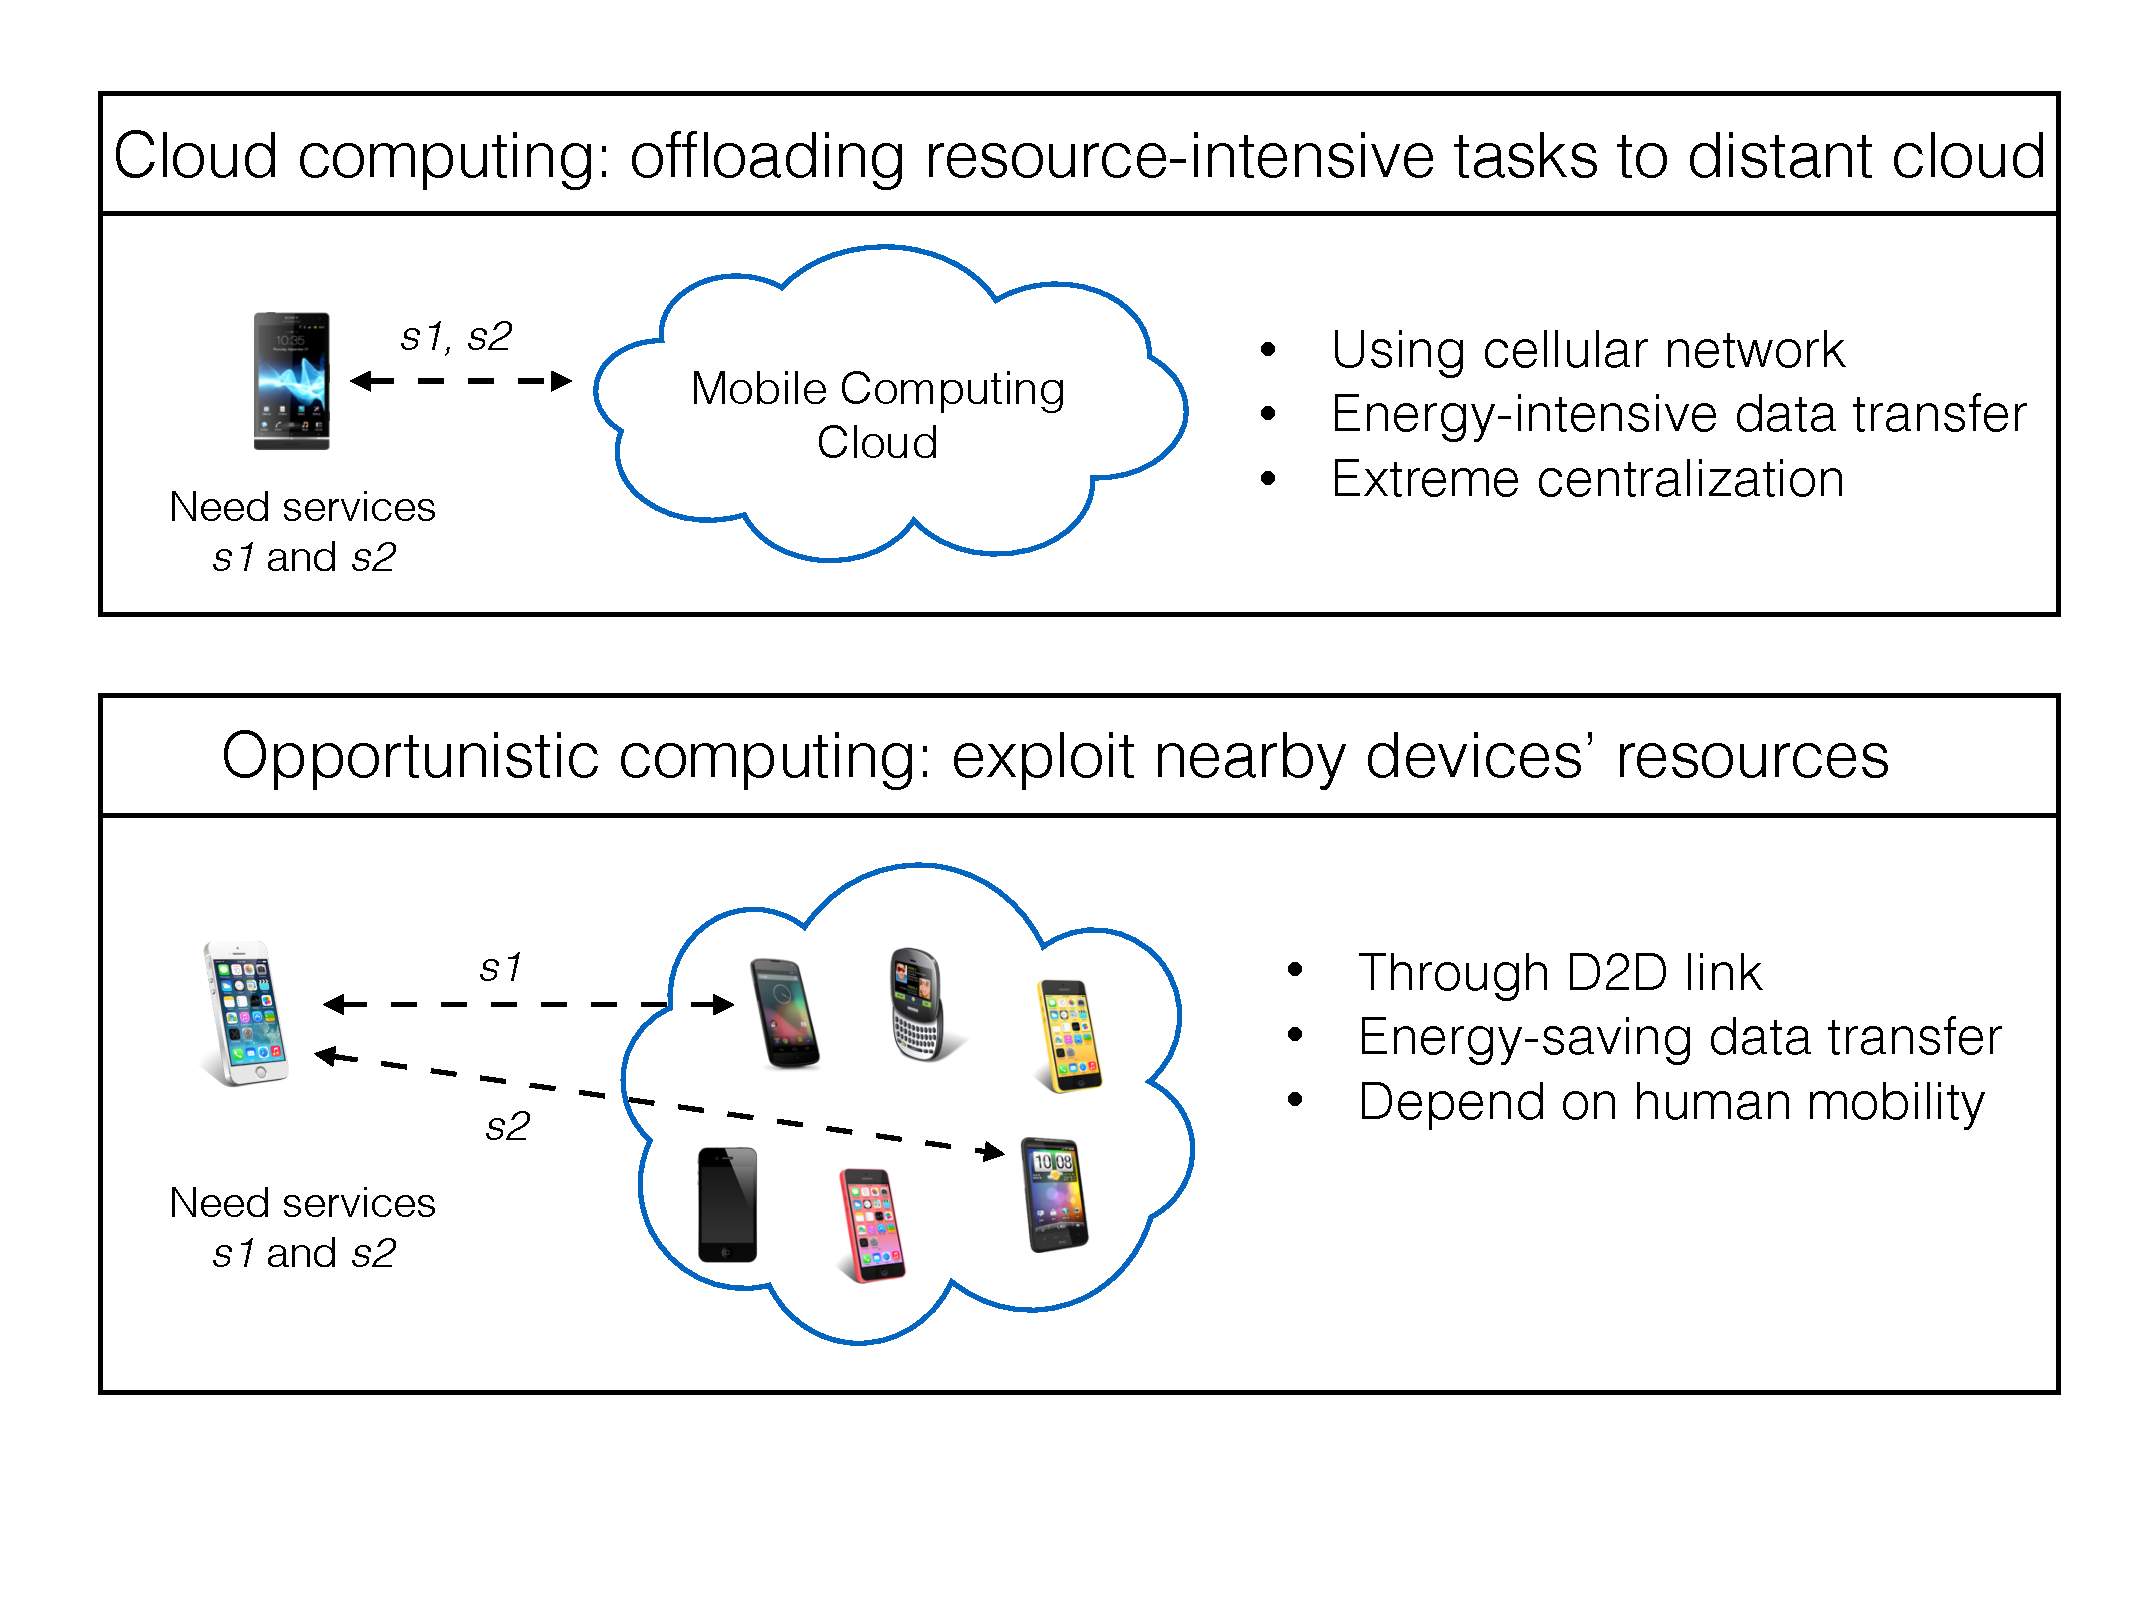
\includegraphics[width=3.5in]{./img/pic1.pdf}
\caption{Opportunistic computing}
\label{Opportunistic computing}
\end{figure}

However, due to the completely different application patterns compared with traditional service computing, service computing in mobile environment faces two inherent challenges.

1) Constant Mobility: Mobile users may change their locations vary frequently in mobile environment, which results in the variation of service availability. Thus, determining how to handle user mobility is a major challenge for providing reliable mobile services in highly dynamic mobile environments.

2) Limited Resource: Mobile devices have limited computing capability compared with other stationary hosts. And mobile service composition schedule must be generated as fast as possible because the availability of mobile service may vary much within a short time. Therefore, how to design a service selection and composition algorithms with fast convergence rate and good scalability is another key challenge.

To address the aforementioned challenges and concerns, we propose an availability-aware mobile service composition approach in this paper, where a mobile user in mobile service opportunistic network are allowed to combine and exploit, through D2D communications, nearby devices' resources with time-varying availability (in contrast, traditional approaches mainly consider fully-available mobile services) to boost their computing power and therefore overcome the limitations of their own resources. 

The main contributions are:

1) We propose a framework (mobile service opportunistic network, MSON in short) to address the problem of service provisioning in the mobile encounter environment where both service requesters and providers are nonstationary and with time-varying availability. In such environment, mobile user can invoke services exposed by nearby mobile devices through D2D links.

2) For MSON, we propose a availability-aware schedule model for service composition to capture users' mobility behavior.

3) Based on MSON and the proposed availability-aware schedule model, we formulate the mobile service composition problem to an optimization problem and propose a Krill-Herd-based algorithm to solve it. 


\section{RELATED WORK}

\subsection{mobile opportunistic network}
Opportunistic networking is one of the most promising evolutions of the traditional multi-hop networking. 
Instead of relying itself on stable end-to-end paths as in the Internet, opportunistic networks do not consider node mobility a problem but as an useful opportunity. 
Marco et al. \cite{Conti2014} give a review of opportunistic network and regarded it as the first step in people-centric networking, they also discuss the focused research problem such as mobility model and routing problem.
Turkes et al. \cite{turkes2016cocoon} proposed a middleware named Cocoon to support mobile opportunistic network, they design a routing protocol above Wi-Fi and Bluetooth standards, their experiments which use real-world data setups show that Cocoon performs well on the aspects of dissemination rate, delivery latency and energy consumption.
Giordano et al. \cite{giordano2011human} proposed a novel paradigm that utilize Opportunistic computing as an appealing complement to the mobile computing cloud, in this way, mobile device can combine and exploit heterogeneous resources from other devices.
Pu et al. \cite{Pu2017crowd} presented QoS-oriented self-organized mobile crowdsourcing framework, in this work, the prevalent and sufficient characteristics of opportunistic user encounters in our daily life are utilized to solve crowdsourcing problem.
Zhan el al. \cite{zhan2017time} propose a time-sensitive incentive-aware mechanism for mobile opportunistic crowdsensing data collection. They formulate the interaction among data carrier and mobile relay users as a two-user cooperative game and apply a asymmetric Nash bargain solution to obtain the optimal cooperation decision and transfer payment.

\subsection{mobile service composition}
Mobile service composition refers to the technique of creating composite services with the help of smaller, simpler and easily executable services or components over mobile networks. Recent technological advances in novel mobile device design and development as well as wireless networking materialize a vision where devices all around a user, either embedded as a part of smart spaces, or being carried by other users
near by, are enabled to present services probably useful. Users sometimes look for services that are not pre-existent on any device but can be dynamically built by appropriately combining already existing ones. For this purpose, extensive research efforts are carried out in this direction. 
For example, Deng et al. \cite{Deng2016} classify mobile service composition methods into three categories: Cloud to Mobile (C2M), Mobile to Mobile (M2M), Hybrid. They also discussed the challenge toward mobile service provisioning and mobile service composition in terms of performance, energy and security perspective. 
Later, Deng et al. \cite{Deng2017} proposed a mobile-service-sharing-community model and extend the random way point (RWP) model to capture user mobility. They utilize the meta-heuristic algorithm to decide the optimal compositional plan. 
Umair Sadiq et al. \cite{sadiq2015service} propose a algorithm for service composition in opportunistic network. They use Levy walk mobility model and SLAW mobility model to represents some scenarios where each node is equally likely to meet any other node. Multi-hops mechanism is used to provides a direct measure for reachability of nodes between devices when an end-to-end connected path does not exist.
Christin Groba et al. \cite{groba2014opportunistic} present a novel service composition protocol that allocates and invokes service providers opportunistically to minimise the impact of topology changes and to reduce failure.
Yang et al. \cite{Yang2010} present a comprehensive QoS model specifically for pervasive services. They consider not only mobile wireless network characteristics but also user-perceived factors. They derive a corresponding formula to calculate the QoS criterion.
zhang et al. \cite{Zhang2016qos} consider a context-aware mobile service selection algorithm based on Genetic Algorithm, They introduce a tree-encoding method to improve the capacity and efficiency of GA. However, for simplicity of the proposed model, they do not consider user mobility.
Wang et al. \cite{wang2011exploiting} model dependable service composition in wireless mobile ad hoc networks by considering mobility prediction of the service providers.
They use a probability-free model and a probabilistic model to characterize the uncertainty of composing. A service that can tolerate a certain level of the mobility of service providers. However, for simplicity of their proposed model, the approach they proposed only apply to the sequential workflows.

It can be seen that the limitation of the existing work lie in: 1) the availability of mobile service is varying fastly in real-world scenario due to the mobility of human. Algorithm which doesn't consider the impact of service availability or consider service availability is full stable may lead to high invoking fail rate, and recompose failed services result in high response time. 2) the work \cite{Deng2017} and \cite{sadiq2015service} consider RWP and  Levy model as mobility model, which borrow concepts and methods from random walks and Brownian motion. However, several studies \cite{barbosa2017human, bettstetter2003node, navidi2004improving} highlighted that individual trajectories are far from random, possessing a high degree of regularity and predictability. And different mobility model applies to different application environment \cite{camp2002survey}, e.g., mobility behavior in a fixed office place is totally different with a crowded subway, thus, it is difficult to find such a model which can apply to every scenario. Therefore, an availability-aware schedule model is more suitable than these long-range mobility model to guide composition schedule to optimal. 
3) some works \cite{wang2011exploiting} \cite{Deng2016-2} use probabilistic model to characterize the uncertainty (i.e, composite service invocation fails because of any one of its concrete service is unavailable). They assume the probability of provider staying within the required distance to the service requester obey a certain rule or distribution. However, in real-world scenario, it is hard to find such a generalized rule or distribution due to different spatial Layout and human traffic (e.g, people flow in a fixed office cubicle is totally different with people flow in a crowded shopping mall). 
The above limitations could be well avoided by using a service availability analysis instead. We therefore introduce an availability-aware schedule model which can better capture users mobility. We then feed a Krill-Herd-based algorithm current availability of candidate services, and generate composition schedule at run-time.

\section{modeling availability-aware mobile service composition}
\begin{figure}[!t]
\centering
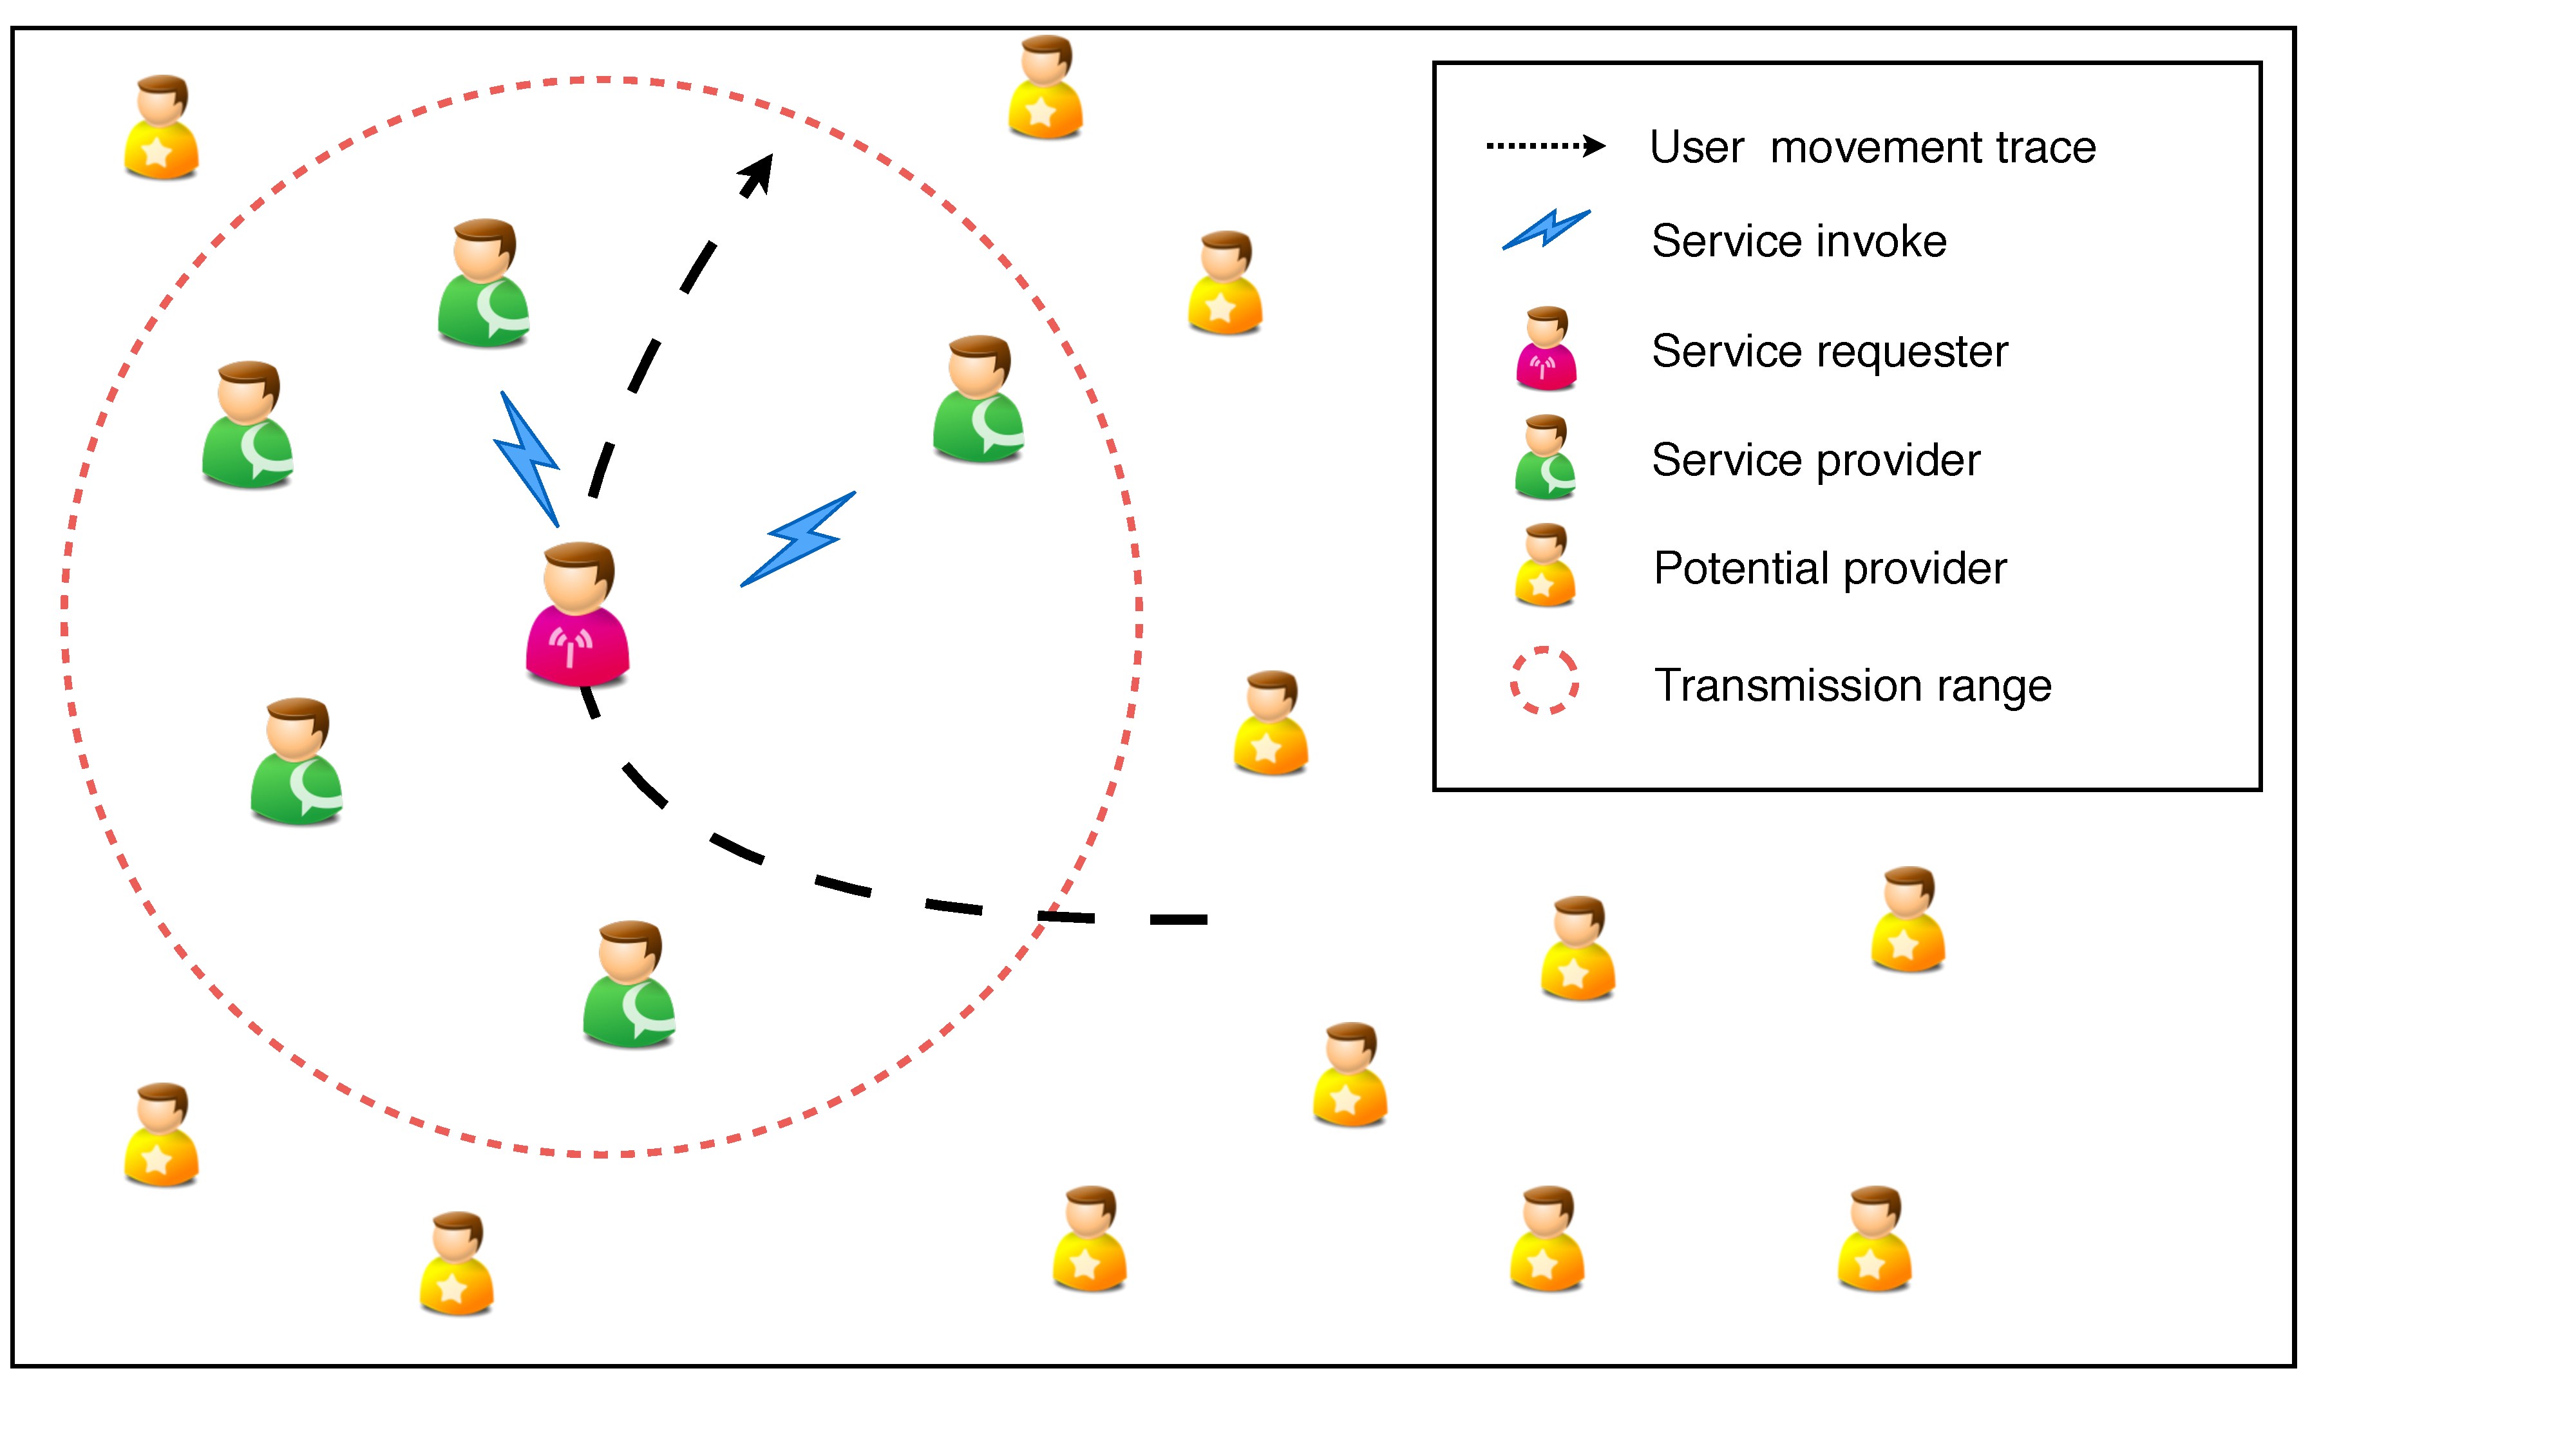
\includegraphics[width=3.5in]{./img/pic2.pdf}
\caption{Mobile service opportunistic network}
\label{fig_mson}
\end{figure}

\subsection{Mobile Service Opportunistic Network Framework}
Fig. 2 illustrates how the mobile services discovery and provision over MSON. In an MSON, a mobile service requester can perceive mobile services exposed by nearby devices through D2D links and launch a composite mobile service (CMS). A composer process, which is in charge of discovering available mobile services nearby, selecting appropriate concrete services, and composing selected services can be implemented and deployed on the mobile device. All concrete services interact with the composer directly.

Note that, we consider only one-hop D2D links for both service requesters and providers. 
Because D2D communications which hops are larger than two would incur network overhead \cite{li2014can} while one-hope communications can lower the delay (e.g., no need to transfer a large volume of task contents hop by hop) and ensure framework choose only local relatively reliable service. 
Besides, some existing researches \cite{chang2015progressive,tuncay2013participant,wu2013homing,jiang2016exploiting,liu2013exploring} reveal that users' one-hop neighbors are sufficient enough, compared with multi-hop mechanisms.

As done by various existing works discussed in the previous section, it is also assumed that MSON has the following properties:

1) Locality: Rather than stable internet, an MSON bases itself on mobile networks and exploits user mobility. Mobile users in MSON can perceive nearby services and establish self-organized local communication within permitted transmission distance.

2) Mobility: Service requesters and providers keep moving in the mobile network even when they are invoking or provisioning mobile services.

3) Dynamicity: Mobile services shared in an MSON are transient because the relative distance between any two services keeps changing and could rise above the permitted transmission distance at any time. 

We use an simple user case to illustrate the related features of service provision over MSON. 
Consider a mobile user who is in a crowded subway and his mobile phone has low battery. 
Now he wants to edit some videos, add some effects and share these video clips to his friends. 
If he do all these operations on his own mobile phone, his mobile phone will run out of energy because of limited battery. 
As one option, he can upload original videos to cloud and use cloud service to get all things done, but offloading task into cloud will result in heavy cellular traffic, which means high energy consumption and expensive communication fee.
But if he is a participant in MSON and several video processing services is provided by some nearby mobile devices, he can invoke such mobile services through D2D communications. 
If these services cannot meet his requirement, several services can be composed. 
Due to users' mobility, the availability of service can vary, invoking mobile services provided by other users may face new challenges that traditional composition methods cannot handle. 
Thus, a mobile service composition model which can capture mobile services' availability need to be proposed.

\subsection{Mobile Service Availability}
\begin{figure}[!t]
\centering
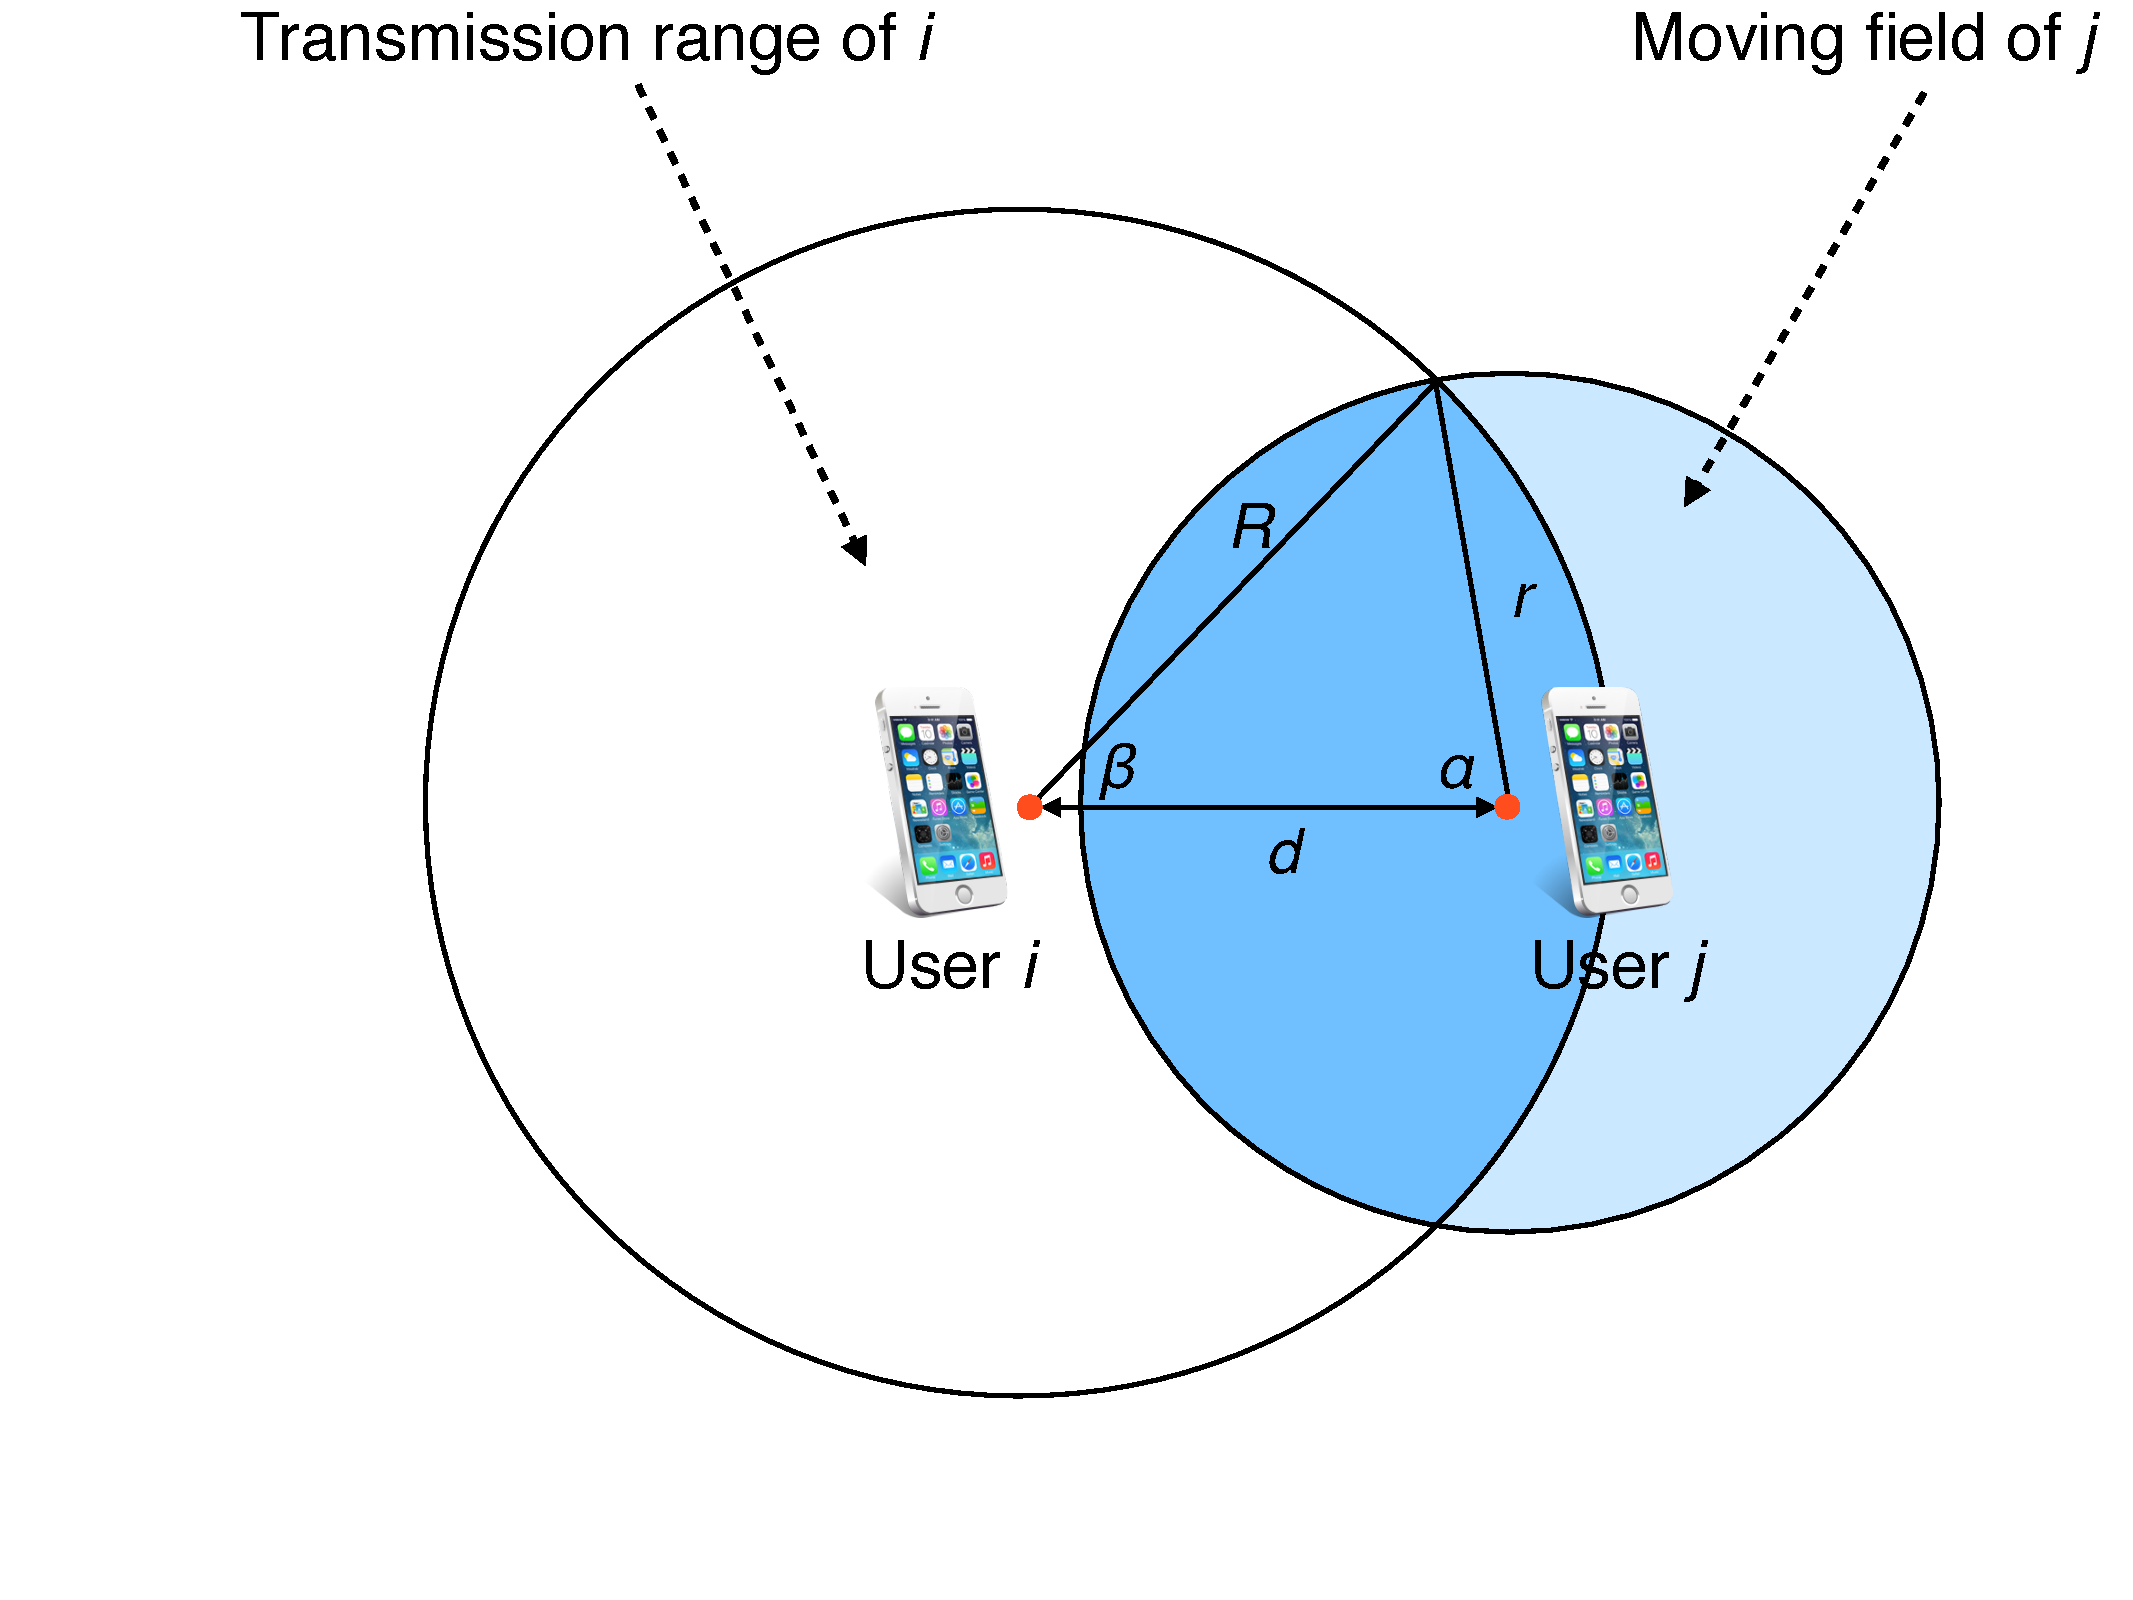
\includegraphics[width=3in]{./img/pic3.pdf}
\caption{Mobile service availability}
\label{fig_sd}
\end{figure}
In an MSON, the availability of mobile service is varying with time and dynamically decided by users' mobility. 
As illustrated by an example in Fig. 3, there are two mobile users $i$ and $j$ with identical transmission rage $R$. User $i$ is a mobile service requester while user $j$ a mobile service provider. Each user moves freely and it is assumed that the moving area is a circle with a radius of $r$ in a certain amount of time, note that this assumption is widely used in related works, e.g., \cite{Yang2010} \cite{wu2001personal}. $d$ is the distance between $i$ and $j$. If user $j$ moves outside the transmission range of its neighbouring user $i$, then user $j$ is unreachable for user $i$ and consequently the services on user $j$ become unavailable to user $i$.

Consider that a mobile service $s$ running on mobile node $j$ is a candidate service for a task requested by user $i$, and the availability of candidate service, $Ava(s)$ can be calculated as the probability that user $j$ keeps staying inside the transmission range of user $i$, it serve as the input into the availability-aware composition model and the scheduling algorithm proposed later:
\begin{equation}
Ava(s) = \frac{S_{i \bigcap j}}{S_j}
\end{equation}
Where $S_{i \bigcap j}$ is the moving area of the user $j$ inside the transmission range of user $i$, $S_j$ the moving field area of the user $j$.

The transmission range of a node $R$ is a preset value (e.g., usually 10m for bluetooth and 25m for Wi-Fi). 
Note that most of wireless transaction protocols have defined the RSSI (Received Signal Strength Indicator), then the distance $d$ between mobile user $i$ and user $j$ can be calculated by signal strength.

The moving radius of a mobile user $r$ is decided by its moving speed $v$ multiplied by the average service time $\bar{t}$. $\bar{t}$ can be statistically calculated as the average service times of recent $n$ trials.
The speed of a mobile user $v$ can be measured and obtained through GPS data or mobile sensors (e.g., Gyro-sensor), then the moving radius can be calculated as the product of $\bar{t}$ and $v$.

Therefore, $S_{i \bigcap j}$ can be calculated as follows:
\setlength{\arraycolsep}{0.0em}
\begin{align}
S_{i \bigcap j} & =  [(\frac{2\alpha}{2\pi} \times \pi r^2)-(\frac{r^2 sin\alpha cos\alpha}{2} \times 2)]\\\nonumber
& \ \ \ \ +[(\frac{2\beta}{2\pi} \times \pi R^2)-(\frac{R^2 sin\beta cos\beta}{2} \times 2)]\\\nonumber
& = \alpha r^2 + \beta R^2 - (r^2 sin\alpha cos\alpha + R^2 sin\beta cos\beta)
\end{align}
\setlength{\arraycolsep}{5pt}
Where
\begin{eqnarray}
\alpha = arccos(\frac{r^2+d^2-R^2}{2r\times d}) \\\nonumber
\beta = arccos(\frac{R^2+d^2-r^2}{2R\times d})
\end{eqnarray}

Finally, $S_j$ can be obtained as:
\begin{align}
S_j & = \pi r^2 \\\nonumber
& = \pi \times (v \times \bar{t})^2
\end{align}

The availability of mobile service $s$ between requester $i$ and provider $j$ thus can be calculated as follow:
\begin{align}
Ava(s) = \frac{\alpha r^2 + \beta R^2 - (r^2 sin\alpha cos\alpha + R^2 sin\beta cos\beta)}{\pi v^2 \bar{t}^2}
\end{align}

\subsection{System Model}
\begin{figure}[!t]
\centering
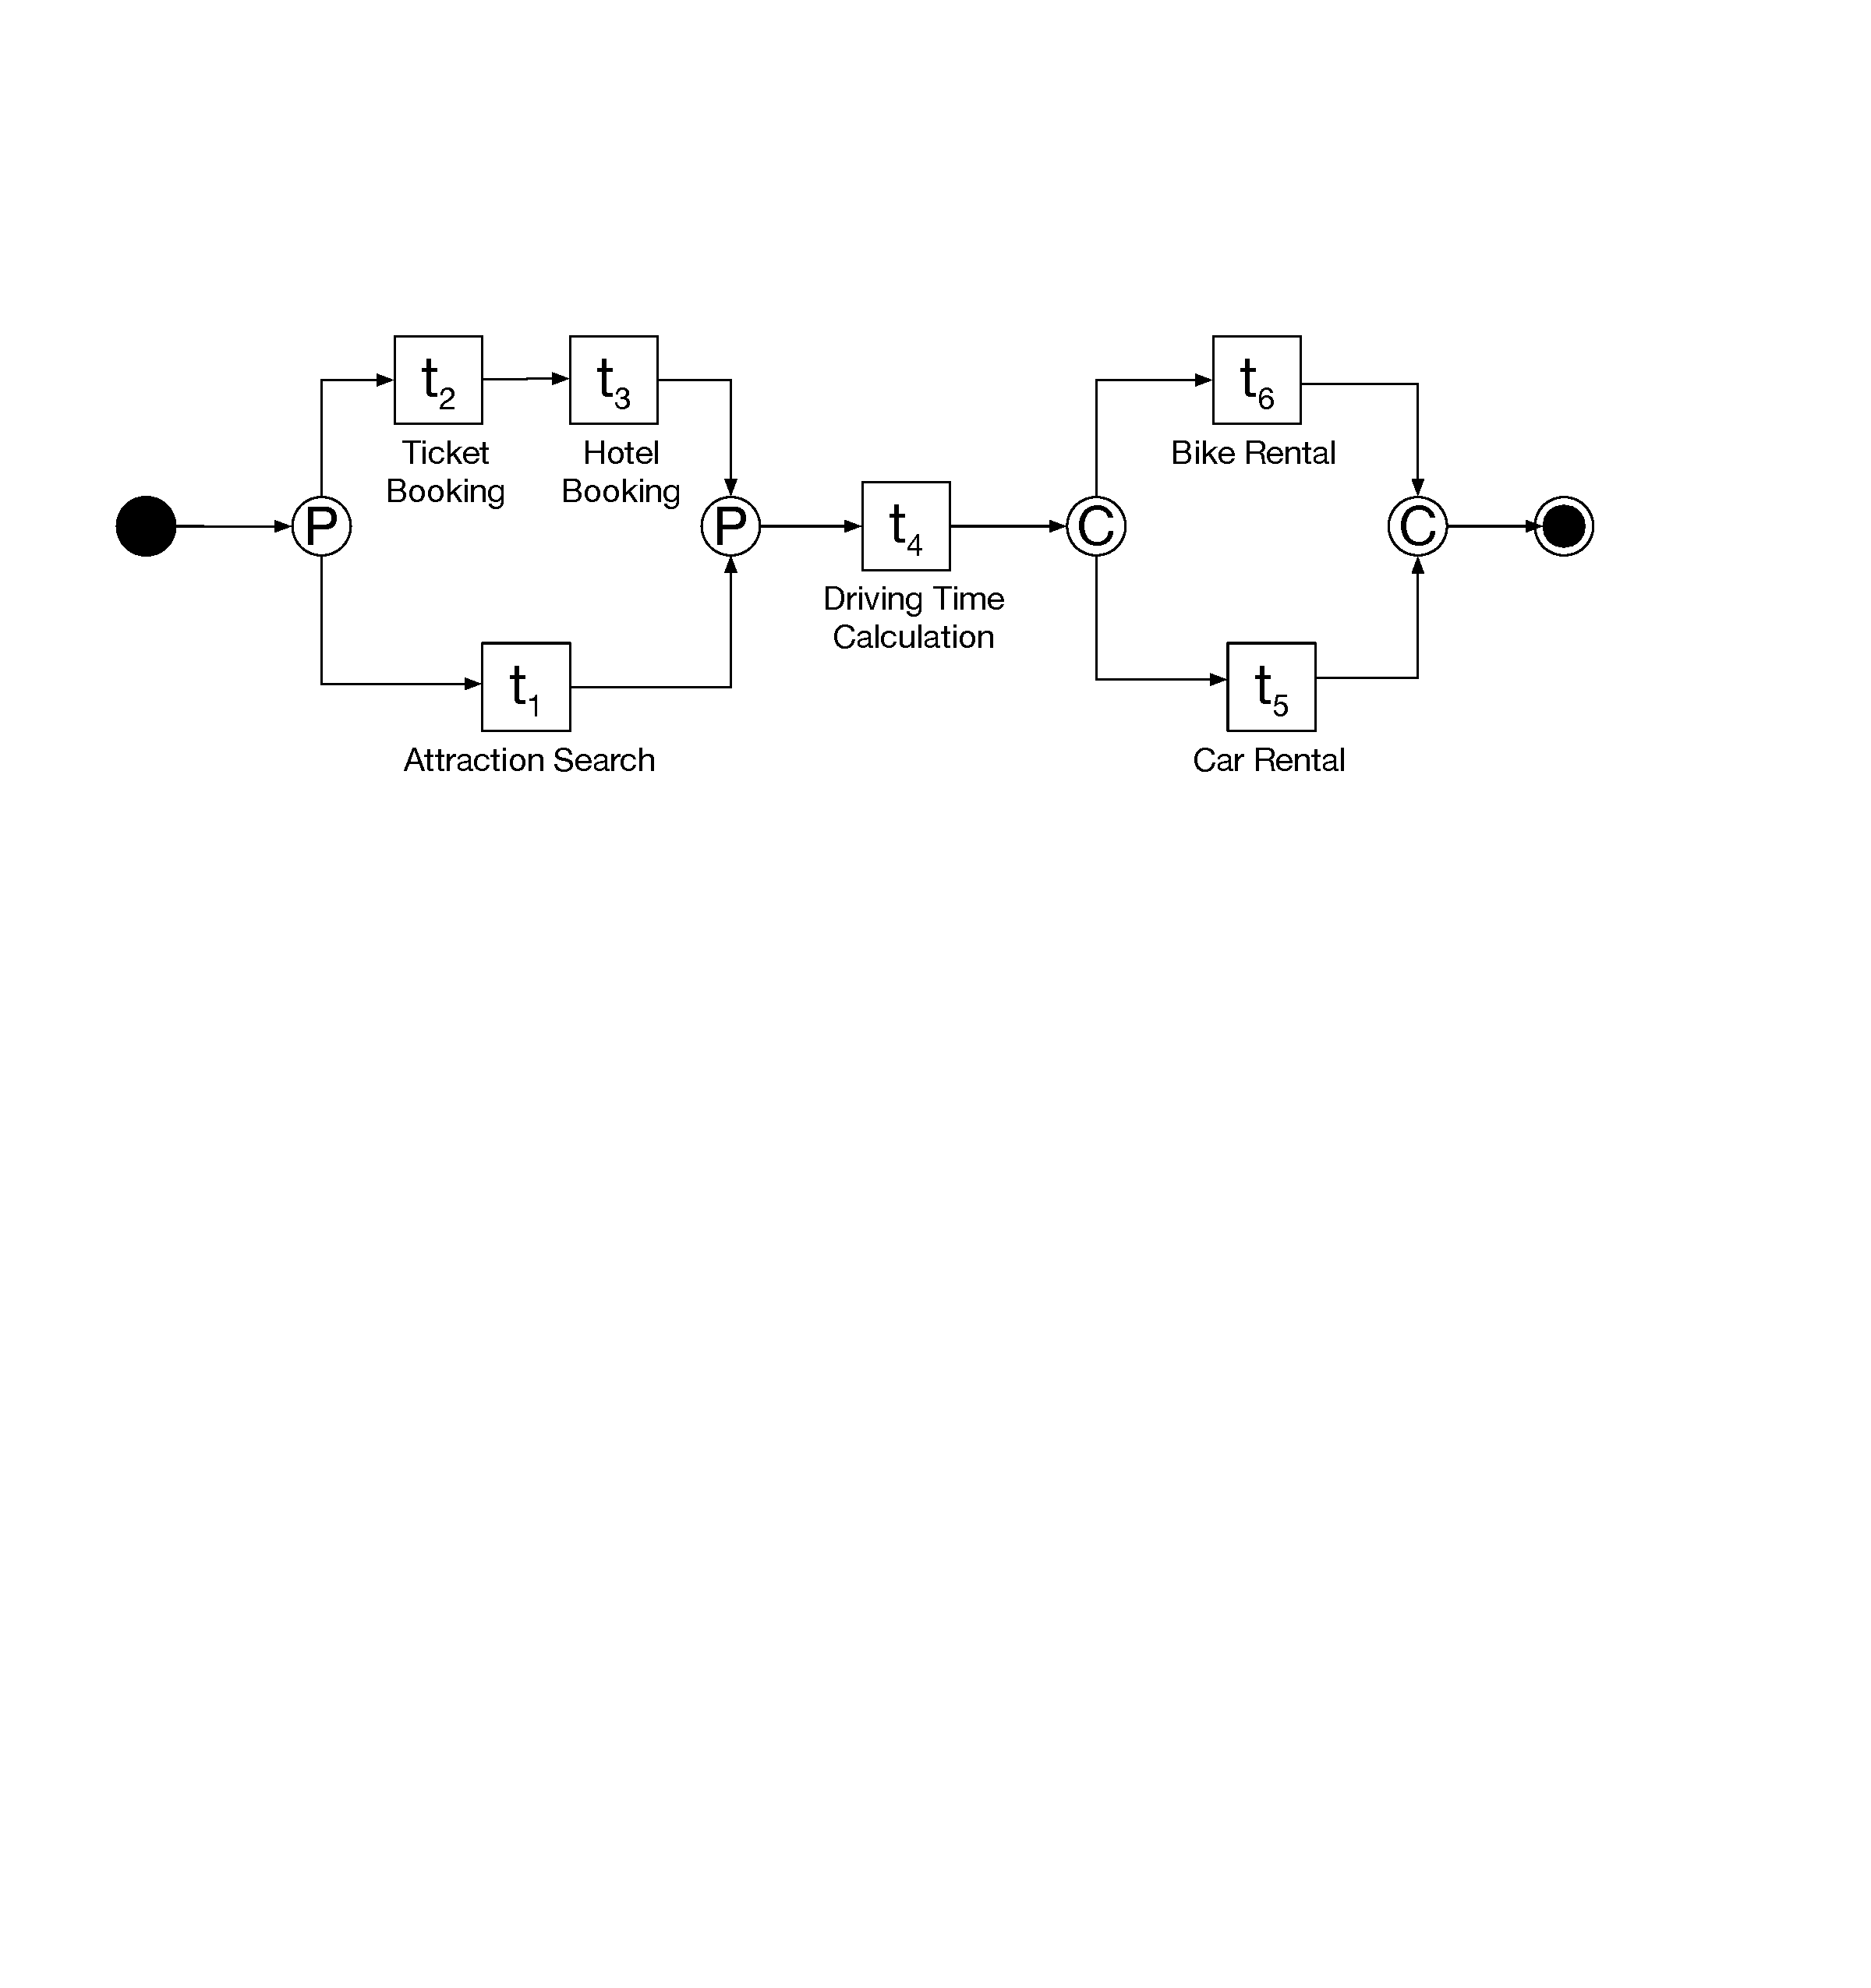
\includegraphics[width=3.5in]{./img/DAG2.pdf}
\caption{A sample composite mobile service for arranging travel}
\label{A sample composite mobile service}
\end{figure}

A composite mobile service (CMS) can be modeled as a workflow $W = (T, E)$ \cite{el2010tqos}, and it is expressed as a directed acyclic graph (DAG), where $T = \{ t_1, t_2, ..., t_n \}$ is a set of tasks and $E$ is a set of directed edges. An edge $e_{i,j}$ of the form $(t_i,t_j)$ indicates that a data dependency between $t_i$ and $t_j$ exists and $t_i/t_j$ are the parent$/$child tasks respectively. A child task is executed after all its parent tasks are completed. 
Furthermore, if there is data transmission $data_{i,j}$ attached onto $e_{i,j}$, then $t_j$ can start only after the data from $t_i$ has been received.
To generalize the workflow with one entry and one exit, two dummy tasks $t_{entry}$ and $t_{exit}$ with zero execution time are added to the beginning and the end of the workflow, respectively. 
A sample composite mobile service for arranging travel is illustrated in Fig. 4. We denote the composition patterns (i.e, sequence, choice, parallel and loop) by symbols $\rightarrow$, \encircle{C}, \encircle{P} and \encircle{L}, respectively.

The execution order of a workflow can be expressed by assigning an index to each task. The index ranges from $1$ to $m$ and the $i$-th item indicates the order of executing $t_i$. The relationship between each task and its index can be described by a function $l : T \rightarrow N^+$ and encoded as a vector containing a permutation of $1$ to $m$. The starting time of tasks is decided by the completion time of their preceding tasks.

A MSON participant can perceive services exposed by other participant and these available service can be described as service pool $P = \{s_1^{(i)}, s_2^{(j)}, ..., s_m^{(k)} \}$, $s_m^{(k)}$ means there are $k$ candidate services for task $t_m$. Once a user initiate a CMS request, tasks in workflow will be scheduled to the service selected from services pool and executed. 

The response time of a CMS request consists of tasks execution time and data transfer time. If task $t_i$ connects $t_k$ through edge $e_{i,k}$ and they are executed by different service providers, the transfer time, $data_{i,k}$, is inevitable because inter-provider data and control signal transfer is required. Otherwise, $data_{i,k} = 0 $ if both tasks are on the same provider.

Tasks in a CMS request are executed by different tasks providers (i.e, different mobile devices) usually exhibit varying performance. Moreover, a task executed by the same provider at different time may exhibit fluctuating performance. In this paper, we use the average execution time of recent $n$ trials to represent expected execution time.

\begin{table}[!t]
\renewcommand{\arraystretch}{1.5}
\caption{Aggregation functions for Reliability}
\label{aggregation functions}
\centering
\begin{tabular}{cc}
\hline
\bfseries Pattern &  \bfseries Reliability \\
\hline
sequence &  $\prod_{i=1}^{n}Ava(s_i)$ \\
parallel &  $\prod_{i=1}^{n}Ava(s_i)$ \\
choice   &  $\sum_{i=1}^{n} p_i \times Ava(s_i)$ \\
loop     &  $[Ava(s_i)]^{k}$ \\
\hline
\end{tabular}
\end{table}


\subsection{Problem Formulation}
Given a CMS request initiated by a MSON participant, perceive nearby services and select suitable concrete services to achieve an optimal service composition schedule with the best response time $RT$ while meeting the service reliability constraint. The resulting problem can therefore be formulated as:
\begin{align}
Min  \ \ \  : \ \ \ & RT   \\\nonumber
s.t \ \ \ : \ \ \ & \tau \le C
\end{align}
Where $C$ denotes the user-recommended constraint of the reliability of the composition schedule, user can make a tread-off between response time and reliability. $\tau$ is the estimated reliability to accomplish the workflow, it can be get by aggregation functions shown in Table 1.

The derivation of $RT$ requires some efforts. $RT$ can be calculated as the estimated ending time of the last task in the CMS workflow:
\begin{align}
\tau = d_m
\end{align}
where $d_i$ denotes the estimated ending time of task $t_i$.

$d_i$ can be iteratively calculated as:
\begin{align}
d_i = e_i + b_i
\end{align}
where $b_i$ denotes the estimated starting time of executing $t_i$ and $e_i$ the execution time of $t_i$ itself.

$b_i$ is decided by the estimated ending time of its immediately preceding tasks and the time required for data transfer. Let $\gamma_i$ denote the estimated time that all earlier tasks scheduled to the same provider to $t_i$ finished, we have:
\begin{align}
\gamma_i =  max\{d_j \mid l(j) < l(i) \wedge w(i) = w(j) \}
\end{align}
where $l(j) < l(i)$ indicates that $t_j$'s order index is smaller than that of $t_i$ and $w(i) = w(j)$ means that $t_i$ and $t_j$ are scheduled into the same provider.

Note that the dependency constraint requires that a task be executed only if its all immediately preceding ones successfully terminate and transfer data. We use $y_i$ to denote the estimated earliest time that the described condition holds for $t_i$.
\begin{align}
y_i = max \{d_k + data_{k,i} \mid t_k \ \in \ ^{*}t_i \} 
\end{align}
where $^{*}t_i$ denotes the immediately preceding tasks of $t_i$ , i.e., those which directly connect $t_i$ through edges in the workflow.
The earliest possible time to execute $t_i$, $b_i$, can therefore be calculated as:
\begin{align}
b_i = max \{ \gamma_i, y_i \}
\end{align}
The entry task of a workflow has no preceding tasks and therefore its estimated ending time is obtained as:
\begin{align}
d_1 = b_1 + e_1
\end{align}
Where $b_1$ can be obtained as:
\begin{align}
b_1 = \delta + data_{entry, 1}
\end{align}
where $\delta$ is the time between initiate a CMS request and a corresponding schedule is generated.

The aforementioned can be reduced to a knapsack problem. It's known that the optimization problem of a knapsack problem is NP-hard \cite{papadimitriou1998combinatorial}, then the problem we formulated is NP-hard.


\section{The kh-based algorithm for mobile service composition}
Because the problem we formulated is NP-hard, there is no known polynomial algorithm which can tell, given a solution, whether it is optimal. Thus, meta-heuristic algorithms such as GA and PSO, can be utilized to find the near optimal solution in polynomial time.

Krill-Herd algorithm \cite{gandomi2012krill} is new generic stochastic optimization approach for the global optimization problem, it is inspired by predatory behavior and communication behavior of krill. 
In this section, we will introduce a Krill-Herd based algorithm to solve the problem of mobile service composition over MSON.

\subsection{Encoding}
In KH, composite service instance is encoded as a krill individual, the krill individual with the best position corresponds to the optimal mobile service composition. The target of algorithm is to find the krill individual with the best position, which means to find the best mobile service composition with the best response time. Therefore, once the optimal krill individual is found, the best mobile service composition is obtained.

In this paper, the position vector of each krill individual is represented by an integer array with its length equal to the number of involved tasks. The $i$-th entry in the array, in turn, refers to the selection result of the task $t_i$ . That is to say, given that the value of the $n$-th entry is $k$, it indicates that $s_{(n,k)}$ is the selected concrete service to execute $t_n$. Fig. 4 illustrates this krill encoding.

\begin{figure}[!t]
\centering
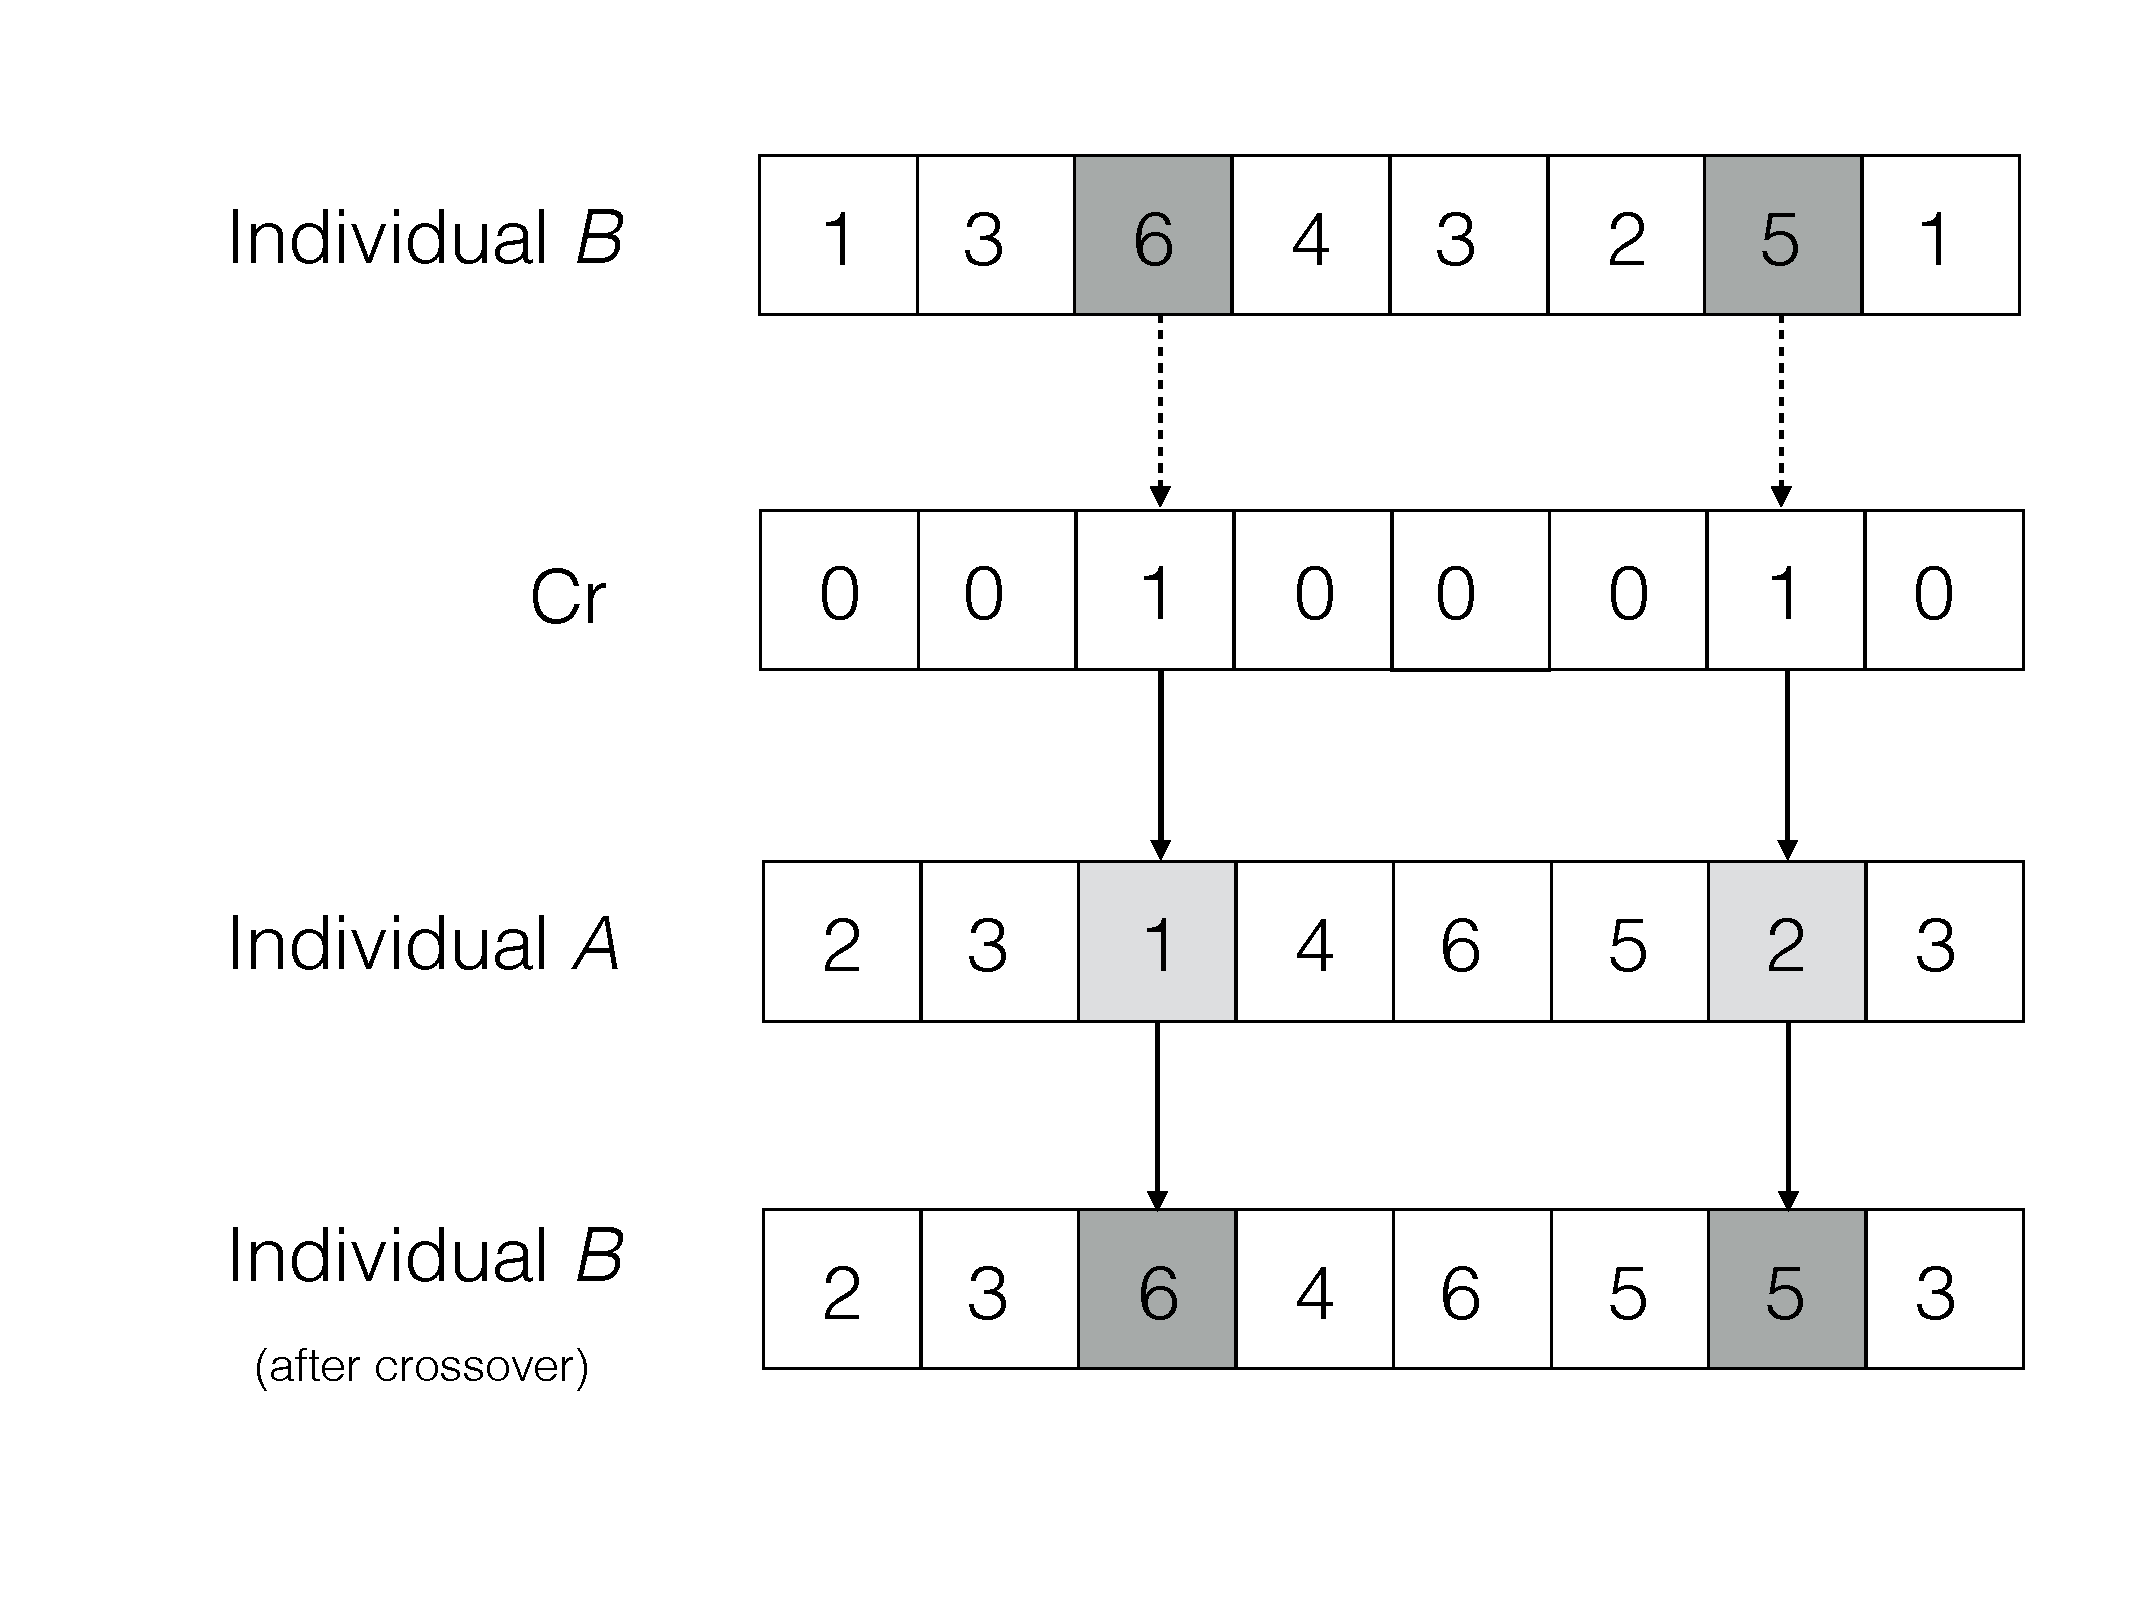
\includegraphics[width=3in]{./img/pic4.pdf}
\caption{Krill encoding}
\label{Krill encoding}
\end{figure}


\subsection{Motion operator}
% 
% 

Motion operator is the key component of KH algorithm. As shown in e.q (11), the position of each krill individual is determined by three main factors: 1) motion influenced by other krill; 2) foraging action; 3) physical diffusion. 
\begin{equation}
\frac{dX_i}{dt} =N_i+F_i+D_i
\end{equation}

where individual $X_i = \{s_{(1,j)}, s_{(2,k)}, . . . , s_{(n,l)}\}$ represents the $i$-th composition service instance in population, $n$ is the number of tasks in the service composition, $N_i$, $F_i$, and $D_i$ denote the motion influenced by other krill individuals, the foraging motion, and the physical diffusion, respectively.

1) Movement induced by other krill individuals

The motion induced by other krill individuals $N_i$ means to learn from neighbor mobile service compositions. It can be formulated as follow:
\begin{equation}
N^{new}_i = N_{max}\alpha_i + \omega_n N^{old}_i
\end{equation}
where
\begin{equation}
\alpha_i = \alpha^{target} + \alpha^{local}
\end{equation}

$\alpha_i$ is the direction of the induced motion and it can be evaluated by target swarm density (target effect $\alpha^{target}$), local swarm density (local effect $\alpha^{local}$). $N_{max}$ is the maximum induced speed, $\omega_n \in [0, 1]$ the inertia weight of the induced motion, $N^{old}_{i}$ is the last induced motion influenced by other krill individuals.

2) Foraging Motion

Similarly, the foraging motion $F_i$ is to learn from the current optimal composite service instance. 
$F_i$ has two parts: the current food location and the information about the previous location. 
For the individual $X_i$, we can formulate this motion as follow:
\begin{equation}
F_i = V_f\beta_i + \omega_f F^{old}_i
\end{equation}
where
\begin{equation}
\beta_i = \beta_i^{food}+\beta_i^{best}
\end{equation}
where $V_f$ is the foraging speed, $\omega_f \in [0, 1]$ is the inertia weight of foraging, and $F^{old}_i$ is the last foraging motion. $\beta_i$ is the direction of the foraging motion.

3) Random diffusion

For individual $X_i$, the physical diffusion is considered to be a random process. This motion includes two components: a maximum diffusion speed and a random directional vector, it can be formulated as follow
\begin{equation}
D_i = D_{max}\delta
\end{equation}
where $D_{max}$ is the maximum diffusion speed and $\delta \in [-1, 1]$ is a random directional vector.

\subsection{Stud selection and crossover operator}

\begin{figure}[!t]
\centering
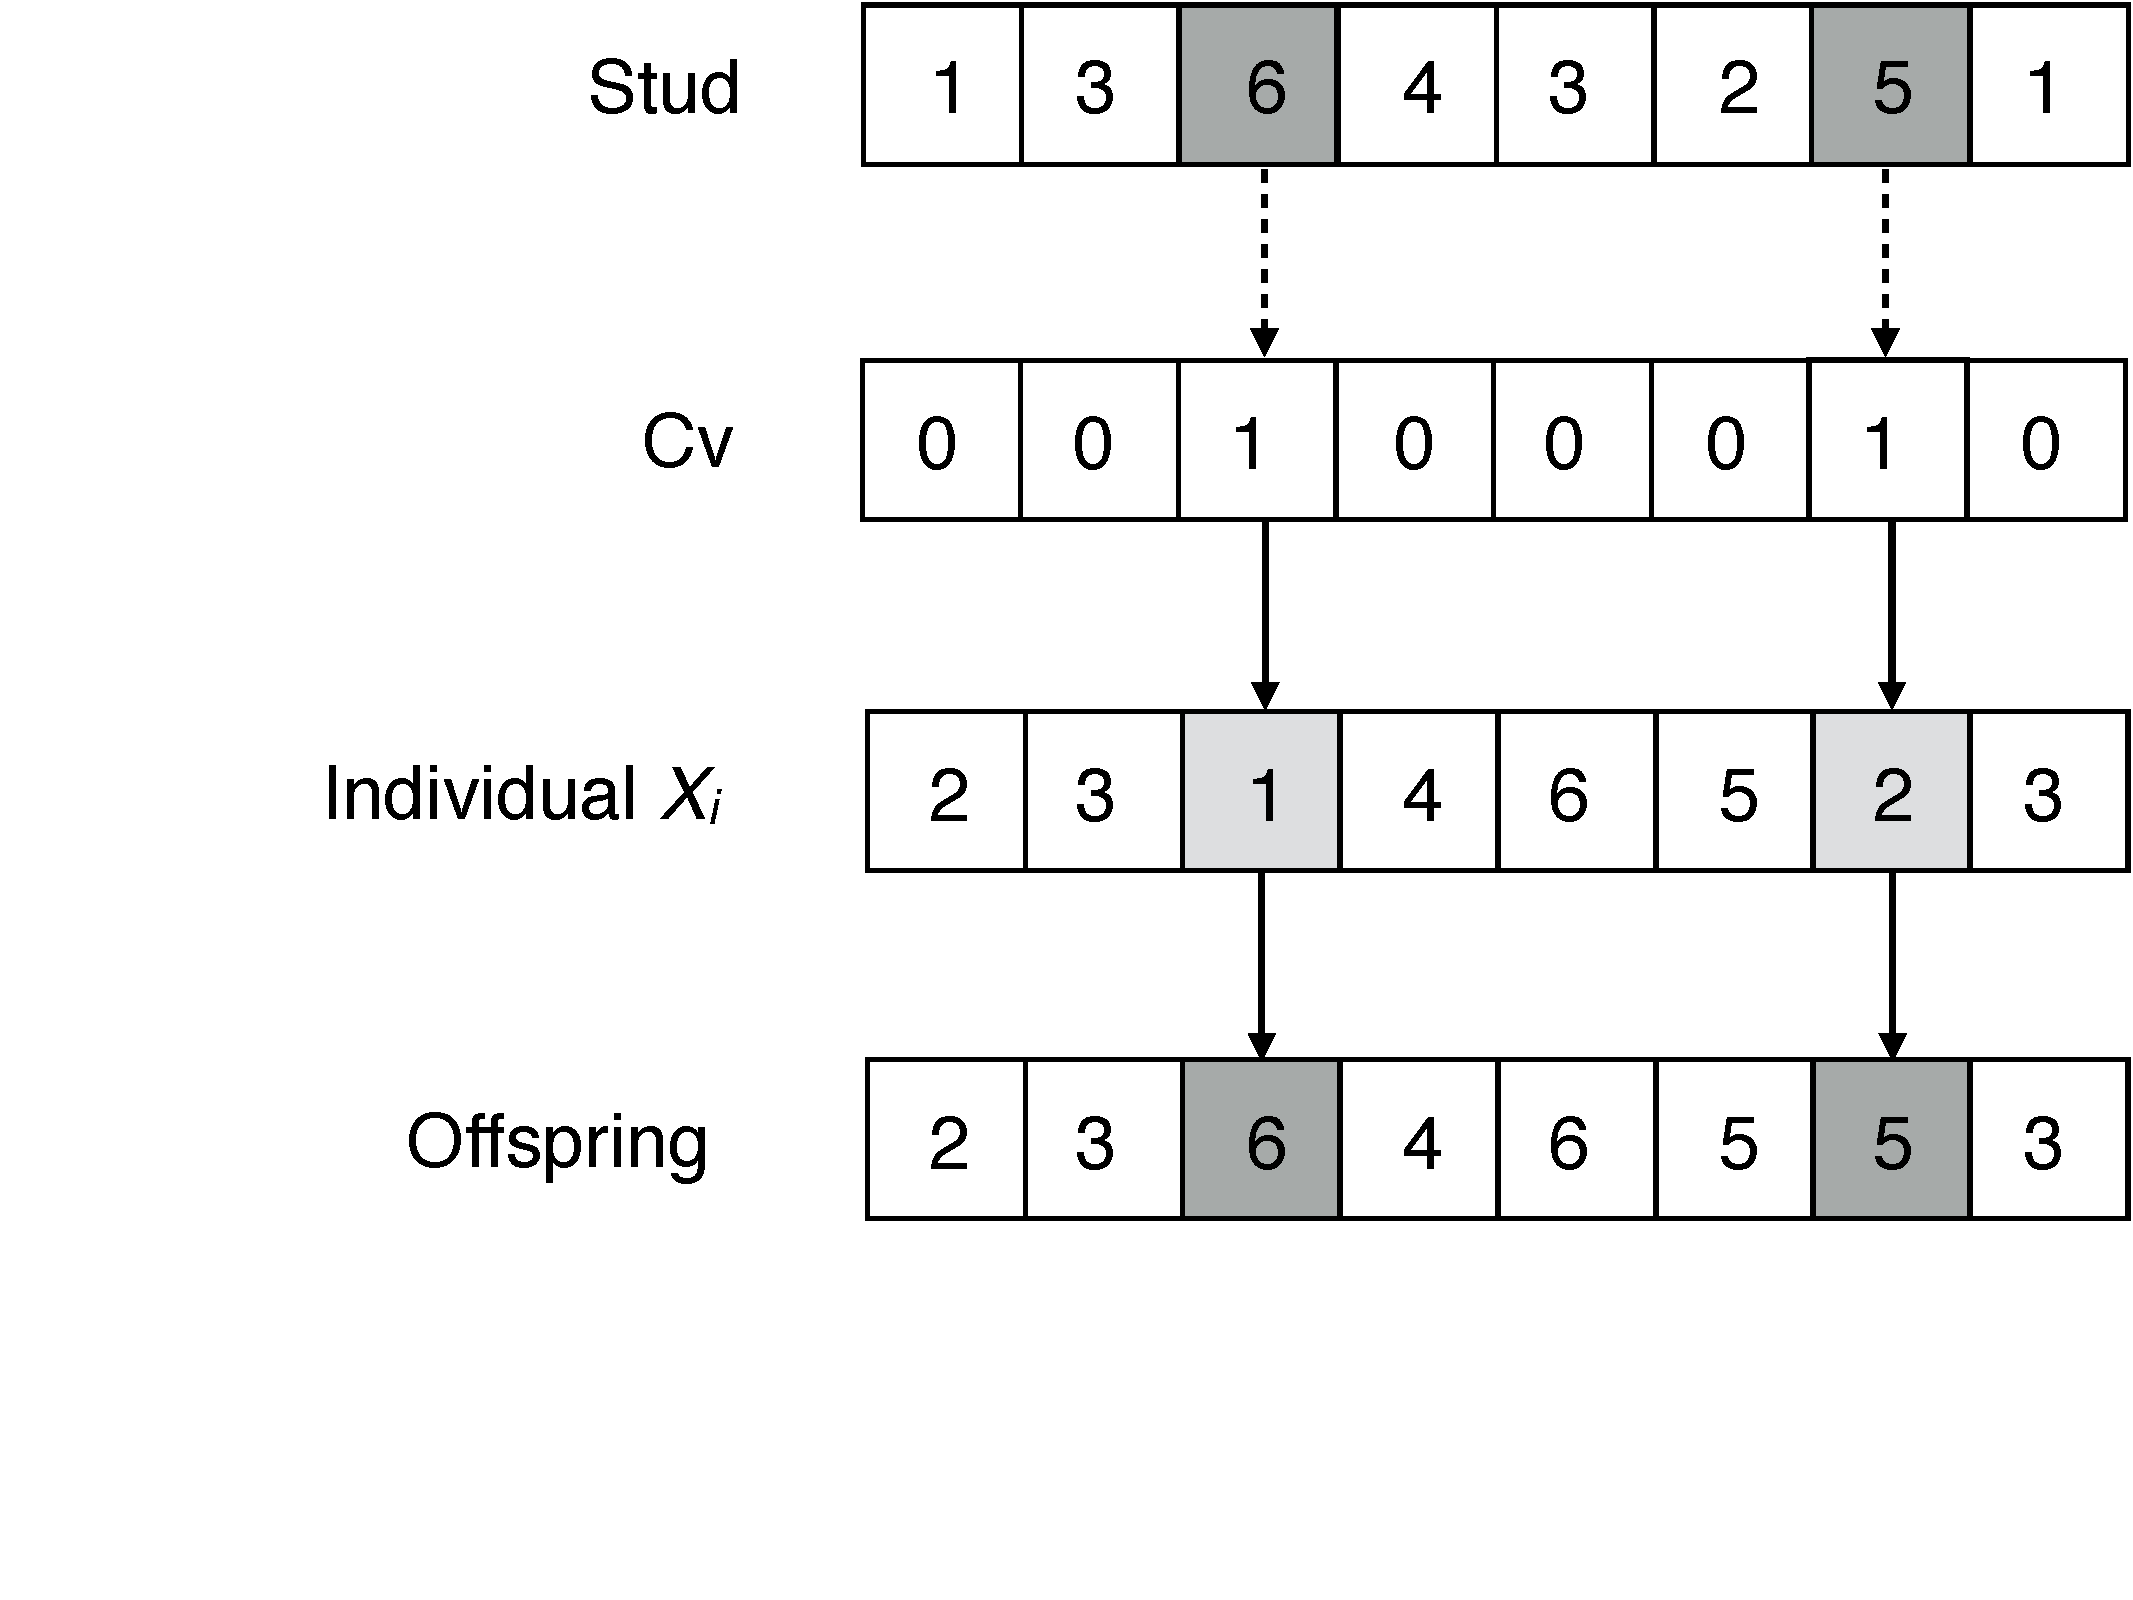
\includegraphics[width=2.5in]{./img/pic5.pdf}
\caption{Crossover operator}
\label{Crossover operator}
\end{figure}


The crossover operator plays an important role in Genetic algorithm for global optimization, we use this operator in KH algorithm to enhance the search capability. The crossover operator in this paper is controlled by a dynamic crossover rate $C_{r}$ which can be obtain as follow
\begin{equation}
C_{r} = r + (1-r) \times \frac{RT_{best}-RT_{i}}{RT_{best}-U_{worst}}
\end{equation}
Where $r$ is a pre-set fixed crossover rate, $RT_{i}$ is the $i$-th individual's response time, $U_{best}$ is the current best response time value, similarly, $U_{worst}$ is the current worst response time value.

Then we can use $C_{r}$ to generate $i$-th individual's crossover vector $Cv = \{c_{1},c_{2},...,c_{n}\}$, it can be manipulated as follows
\begin{equation}
c_{i}=
\begin{cases}
1,& if \ \ rand(0,1) < C_{r}\\
0,& else\\
\end{cases}
\end{equation}
Inspired by SGA \cite{wang2014stud} (a type of GA which employs the optimal genome for crossover at each generation), we introduce stud selection procedure to improve KH's search capability.
From algorithm 1, we can see that for each individual $X_i$ to crossover, we choose the optimal individual $Stud$ (i.e., the individual with best response time value) to mating. As shown in Fig. 7, the characteristics from individual $Stud$ are copied to individual $X_i$ according to crossover vector $Cv$. 

\begin{algorithm}
\caption{Crossover operation}
\label{alg1}
\begin{algorithmic}[1]

\REQUIRE Population $X$; Individual $X_i$ to crossover; The number of tasks $taskNumber$; 
\STATE Sort all krill individuals in population $X$ by its response time, get optimal individual $Stud$, save the best response time value as $RT_{best}$ and the worst response time value as $RT_{worst}$
\STATE $C_{r} \leftarrow$ calcCrossoverRate($X_i$, $RT_{best}$, $RT_{worst}$)
\FOR{$i=0$ \TO $taskNumber$}
\STATE $r \leftarrow rand(0,1)$
\IF{$r < C_{r}$}
\STATE $Cv[i] \leftarrow 1$
\ELSE
\STATE $Cv[i] \leftarrow 0$
\ENDIF
\ENDFOR
\FOR{$i=0$ \TO $taskNumber$}
\STATE $X_i[i] \leftarrow X_i \wedge  (1-Cv[i]) + Stud \wedge Cv[i]$ 
\ENDFOR
\end{algorithmic}
\end{algorithm}

\subsection{Update position}
After crossover, the offspring should be evaluated and updated to current evolutionary sequence.
According to the three motion actions, the time-relied position from time $t$ and $\Delta t$ can be formulated by the following equation
\begin{equation}
X_{i+1} = X_i + \Delta t \frac{dX_i}{dt}
\end{equation}

where
\begin{equation}
\Delta t = C_t\sum_{j=1}^{n}(UB_j - LB_j)
\end{equation}

where $n$ is the tasks number of composition service, $UB_j$ and $LB_j$ are upper and lower bounds of candidate services for the $j$-th task, respectively. $C_t$ is a constant value to scale the searching space and we set it to $1/2n$ in this paper. Finally, the overall KH algorithm process can be describe in Algorithm 2.

\begin{algorithm}
\caption{KH algorithm}
\label{alg2}
\begin{algorithmic}[1]

\REQUIRE Number of population size $PS$, Number of max iteration $MI$;

\STATE Generate initial population as $X = (X_1, X_2, ..., X_{PS})$
\STATE estimate response time of each krill individual in $X$
\FOR{$i=0$ \TO $MI$}
  \FOR{$i=0$ \TO $PS$}
    \STATE $X_i^{'} \leftarrow motionOperator()$
    \STATE $X_i^{''} \leftarrow crossoverOperator(X_i^{'})$
    \STATE $RT_i^{'} \leftarrow estimateResponseTime(X_i^{'})$
    \STATE $RT_i^{''} \leftarrow estimateResponseTime(X_i^{''})$
    \IF{$RT_i^{''} < RT_i^{'}$}
      \STATE update position by e.q (24) as $X_{i+1}$
    \ELSE
      \STATE accept $X_i^{''}$ as $X_{i+1}$
    \ENDIF
  \ENDFOR
\ENDFOR
\STATE Output the best solution
\end{algorithmic}
\end{algorithm}


\section{SIMULATION AND EVALUATION}
In this section, we first discussed the experimental environment settings, then we evaluate the impact of parameters and compare our algorithm with other non-availability algorithms in terms of success rate and response time.

\subsection{Simulation Setting}
To evaluate the optimality and scalability of the proposed approaches, the experiment is run on a personal computer with an Intel Core i5 CPU with 2.4 GHz, 4 GB RAM, macOS and Matlab R2015b Edition.

Since we can not find available realistic datasets which involving both user D2D contact traces and quality of mobile service so far, we attempt to simulate the scenarios for mobile services provision by integrating realistic user D2D contact traces with quality of Web service datasets. 

We consider MIT Reality dataset \cite{eagle2006reality} as user D2D contact traces, where user location, Bluetooth devices in proximity, application usage, and phone status (such as charging and idle) were collected from 100 users over several months. This dataset can really reflect diverse network scenarios.

The publicly available quality of Web service (QWS) dataset\cite{zheng2014investigating} can be used to characterize the service candidates. This dataset consists of 4500 Web services from 142 users over 64 different time slices (at 15-minute interval) and each QoS data includes two measurements (response time and throughput).
% for a mobile service, response time attribute is randomly selected from the QWS dataset. 

\begin{table}[!t]
\renewcommand{\arraystretch}{1.5}
\caption{User $u$ 's D2D contract traces}
\label{D2D contract traces}
\centering
\begin{tabular}{c c}
\hline
\bfseries Time & \bfseries Available service provider\\
% user(3).devices_names(500-505)
% \hline
\hline
t1 & Rabbit, Tony, S10, BlueRadios, NORTHOLT\\
% \hline
t2 & Tony, S10, Rabbit, NORTHOLT, BlueRadios\\
% \hline
t3 & Rabbit, NORTHOLT, BlueRadios, S10, Tony, Henrymobile, S4 \\
% \hline
t4 & Tony, NORTHOLT, BlueRadios, S10, Rabbit, S4\\
% \hline
t5 & BlueRadios, S4, AliKatz, NORTHOLT, Rabbit, S25, S10\\
% \hline
t6 & S25, S10, NORTHOLT, BlueRadios, Rabbit\\
% \hline
... & ...\\
\hline
\end{tabular}
\end{table}

\begin{table}[!t]
\renewcommand{\arraystretch}{1.3}
\caption{Services exposed by provider}
\label{Services exposed by provider}
\centering
\begin{tabular}{c c}
\hline
\bfseries Service Provider & \bfseries Exposed Service\\
% user(3).devices_names(500-505)
\hline
% \hline
AliKatz     & $s_1$, $s_2$, $s_3$, $s_4$\\
% \hline 
BlueRadios  & $s_1$, $s_5$\\
% \hline
Henrymobile & $s_2$, $s_4$\\
% \hline
NORTHOLT    & $s_4$, $s_5$, $s_6$ \\
% \hline
Rabbit      & $s_1$, $s_4$\\
% \hline 
S4          & $s_1$, $s_2$\\
% \hline 
S10         & $s_6$, $s_7$\\
% \hline 
S25         & $s_4$, $s_5$\\
% \hline 
Tony        & $s_1$, $s_4$\\
% \hline 
... & ...\\
\hline
\end{tabular}
\end{table}

\begin{table}[!t]
\renewcommand{\arraystretch}{1.8}
\caption{Available candidates}
\label{Available candidates}
\centering
\begin{tabular}{c c}
\hline
\bfseries Time & \bfseries Available service\\
% user(3).devices_names(500-505)
\hline
% \hline
t1     & $s_1^{(3)}$, $s_4^{(3)}$, $s_5^{(2)}$, $s_6^{(1)}$, $s_7^{(1)}$ \\
% \hline 
t2     & $s_1^{(3)}$, $s_4^{(3)}$, $s_5^{(2)}$, $s_6^{(2)}$, $s_7^{(1)}$ \\
% \hline
t2     & $s_1^{(4)}$, $s_2^{(2)}$, $s_4^{(4)}$, $s_5^{(2)}$, $s_6^{(2)}$, $s_7^{(1)}$ \\
% \hline
t4     & $s_1^{(4)}$, $s_2^{(1)}$, $s_4^{(3)}$, $s_5^{(2)}$, $s_6^{(2)}$, $s_7^{(1)}$ \\
% \hline
t5     & $s_1^{(4)}$, $s_2^{(2)}$, $s_3^{(1)}$, $s_4^{(4)}$, $s_5^{(3)}$, $s_6^{(2)}$, $s_7^{(1)}$ \\
% \hline 
t6     & $s_1^{(2)}$, $s_4^{(3)}$, $s_5^{(3)}$, $s_6^{(2)}$, $s_7^{(1)}$ \\
% \hline 
... & ...\\
\hline
\end{tabular}
\end{table}

Table 2 is part of D2D contract traces in MIT Reality dataset. For example, there there are five nearby devices within D2D transmission distance at time $t1$ and these devices can be regarded as MSON participant who provision mobile services. Table 3 shows MSON participants and the services they exposed to nearby devices. These mobile service are random chosen from QWS dataset. Table 4 is the Cartesian product of Table 2 and Table 3, it shows how many kinds of services user can exploit at a certain time and how many candidates for each kind of service (i.e., task). For example, there are five kinds of service available at time $t1$ and there are three candidates for task $t_1$, three candidates for task $t_4$, two candidates for task $t_5$, one candidate for task $t_6$ and one candidate for task $t_7$.

\subsection{Impact of Parameters}
\begin{table}[!t]
\renewcommand{\arraystretch}{1.3}
\caption{parameters configuration}
\label{table_example}
\centering
\begin{tabular}{cccccc}
\hline
\bfseries $PS$ & \bfseries $MI$ & \bfseries $CR$ & \bfseries $V_f$ & \bfseries $N_{max}$ & \bfseries $D_{max}$ \\
\hline
1$\sim$60 & 50          & 0.6            & 0.8            &  0.3            &  0.2 \\
20        & 10$\sim$150 & 0.6            & 0.8            &  0.3            &  0.2 \\
20        & 50          & 0.01$\sim$1.00 & 0.8            &  0.3            &  0.2 \\
20        & 50          & 0.6            & 0.01$\sim$3.00 &  0.3            &  0.2 \\
20        & 50          & 0.6            & 0.01           &  0.01$\sim$2.00 &  0.2 \\
20        & 50          & 0.6            & 0.01           &  0.3            &  0.01$\sim$3.00 \\
\hline
\end{tabular}
\end{table}

There are six parameters can be adjusted to improve the KH's performance: population size $PS$, maximum iteration number $MI$, crossover rate $Cr$, foraging speed $V_f$, maximum induced speed $N_{max}$ and physical diffusion speed $D_{max}$. As shown in Table 5, we generate six groups of parameters configuration to evaluate the impact of each parameter. For each group of parameters configuration, we tune one parameter and fix the other parameters. For each configuration setting, the KH algorithm was executed 50 times independently and the average performance was recorded.

\begin{figure*}[!t]
\centering

\subfloat[]{
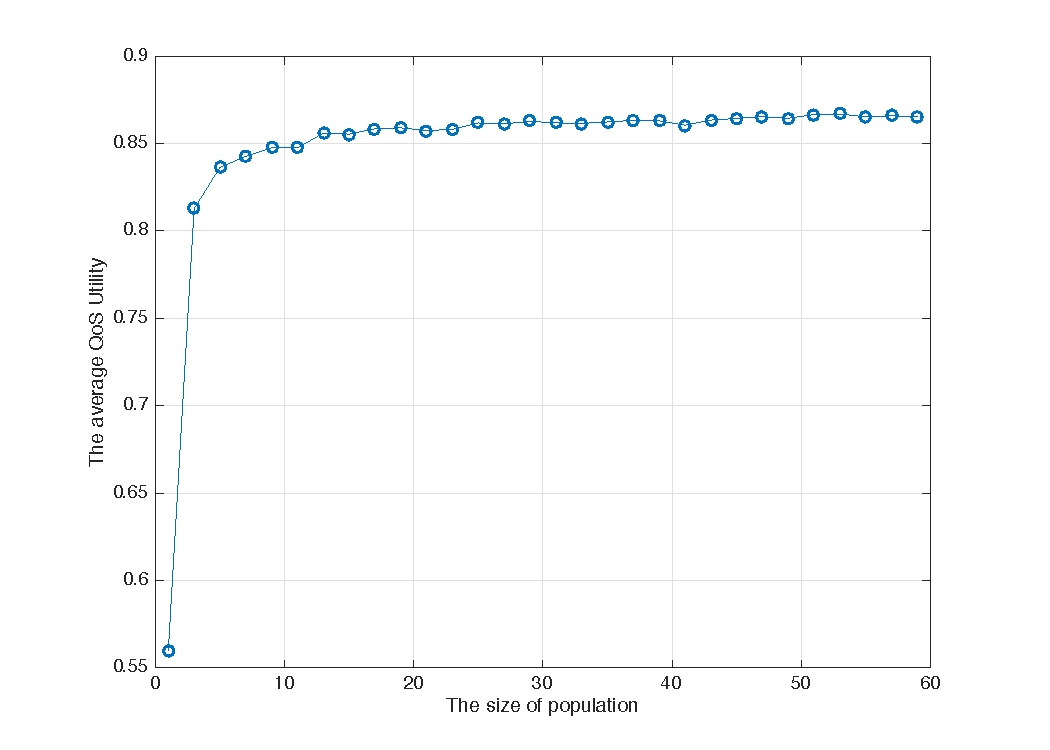
\includegraphics[width=2in]{./img/Param-PS.pdf} 
\label{PS}}
\hfil
\subfloat[]{
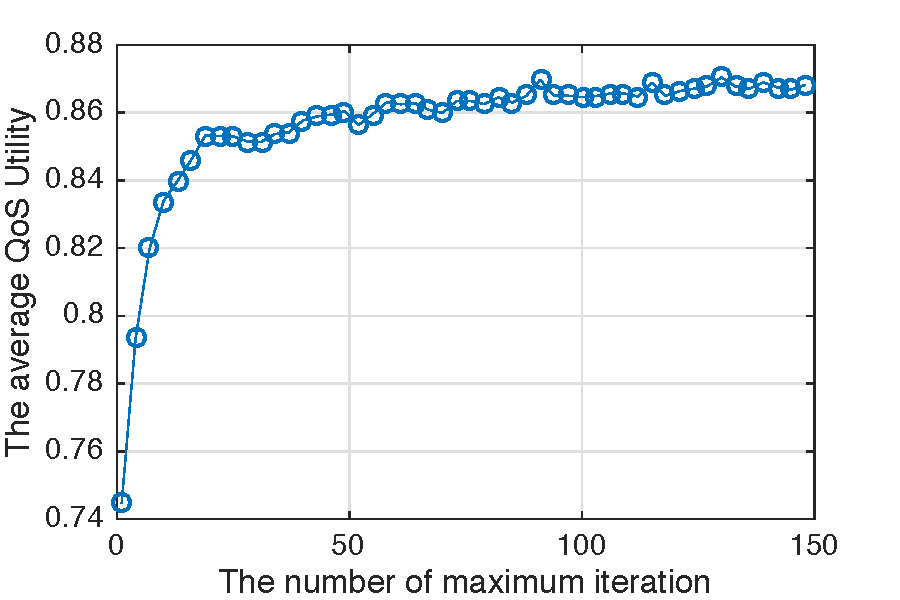
\includegraphics[width=2in]{./img/Param-MI.pdf} 
\label{MI}}
\hfil
\subfloat[]{
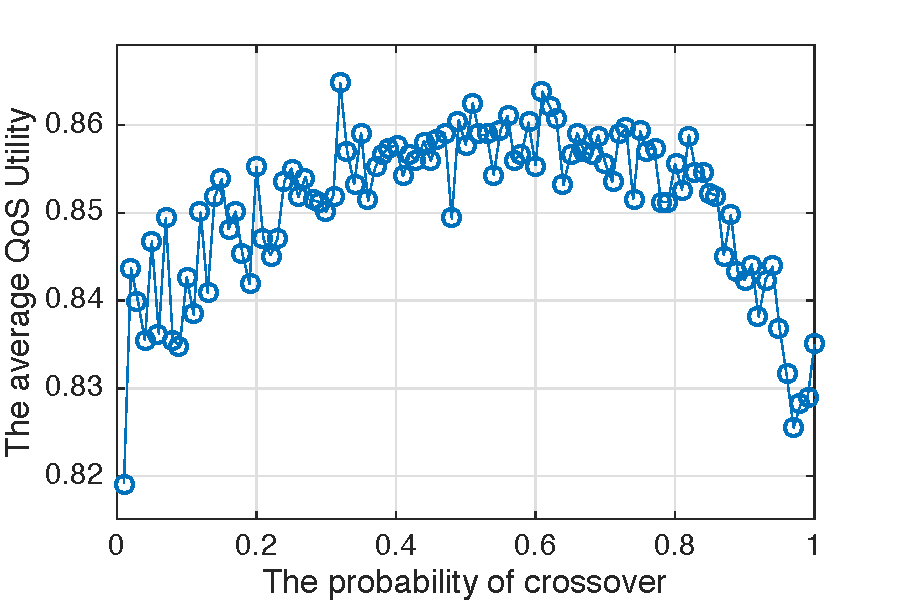
\includegraphics[width=2in]{./img/Param-CR.pdf} 
\label{CR}
}

\subfloat[]{
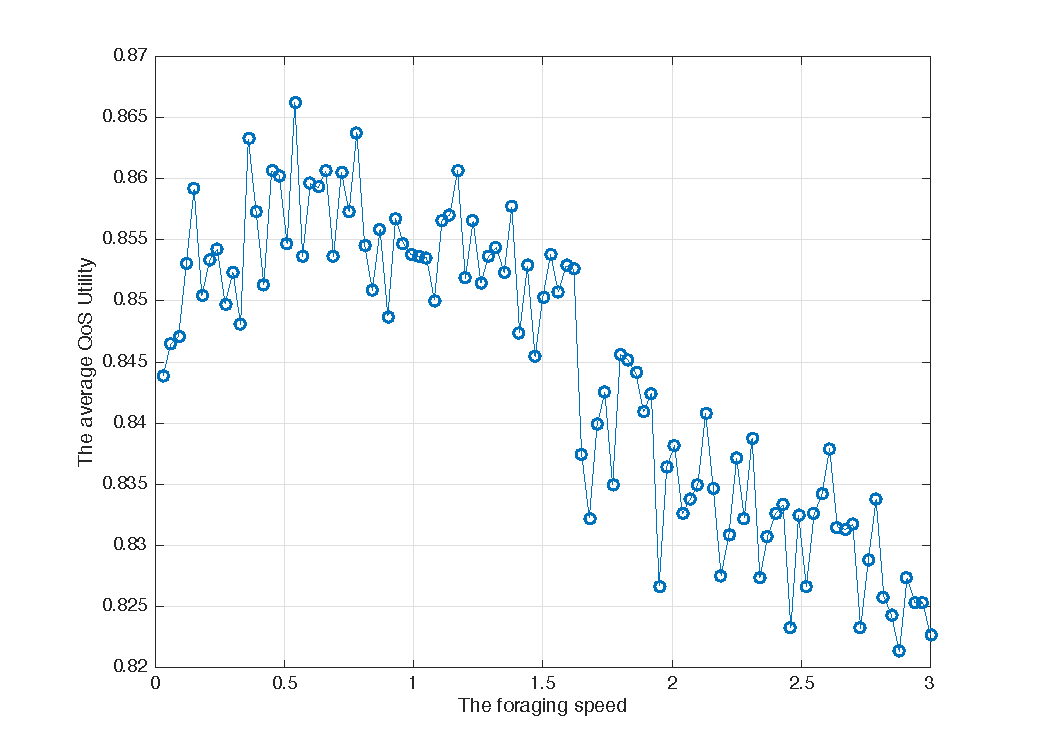
\includegraphics[width=2in]{./img/Param-Vf.pdf} 
\label{Vf}}
\hfil
\subfloat[]{
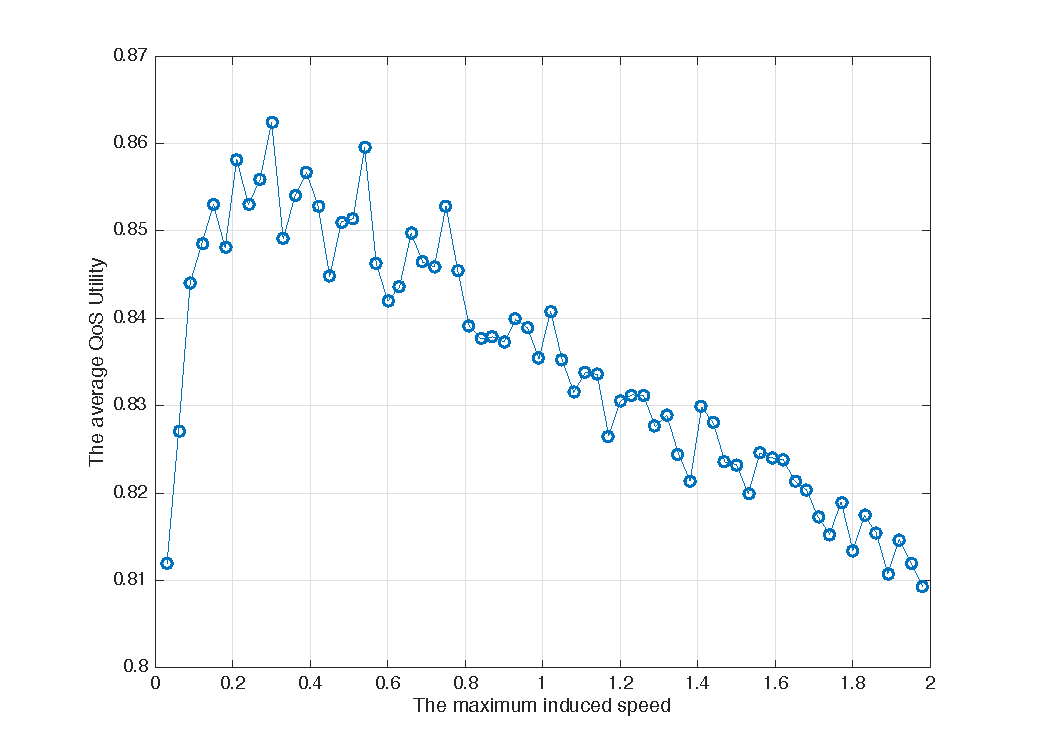
\includegraphics[width=2in]{./img/Param-Nmax.pdf} 
\label{Nmax}}
\hfil
\subfloat[]{
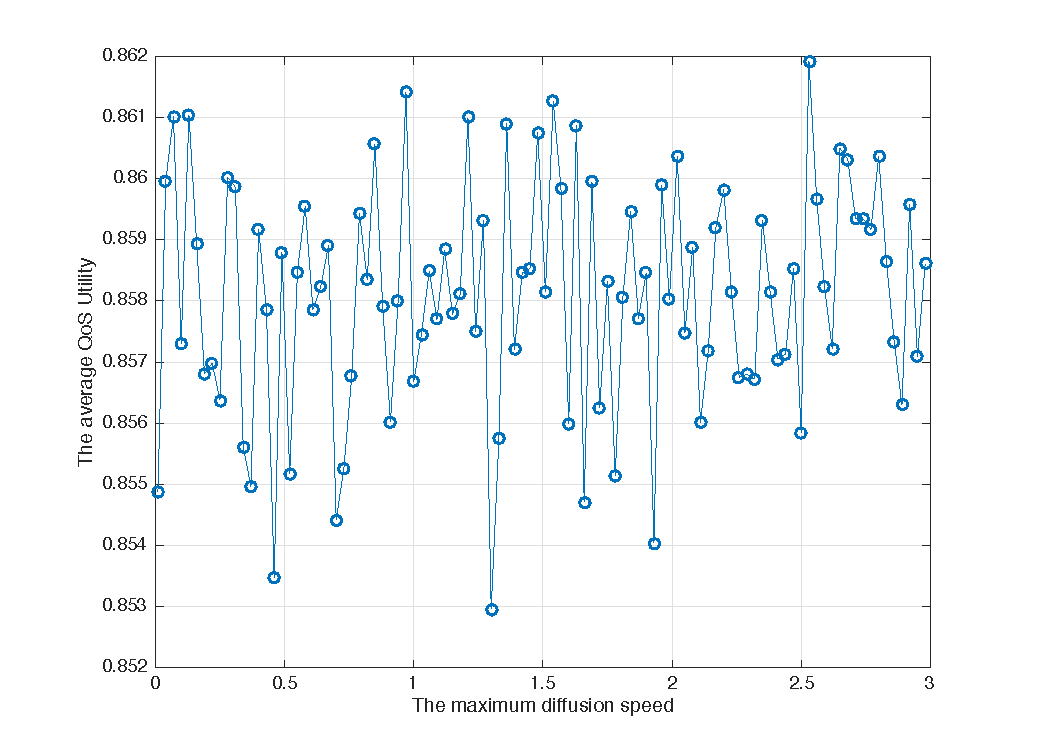
\includegraphics[width=2in]{./img/Param-Dmax.pdf} 
\label{Dmax}}

\caption{Impact of parameters.} \label{fig_sim}
\end{figure*}

\begin{figure*}[!t]
\centering
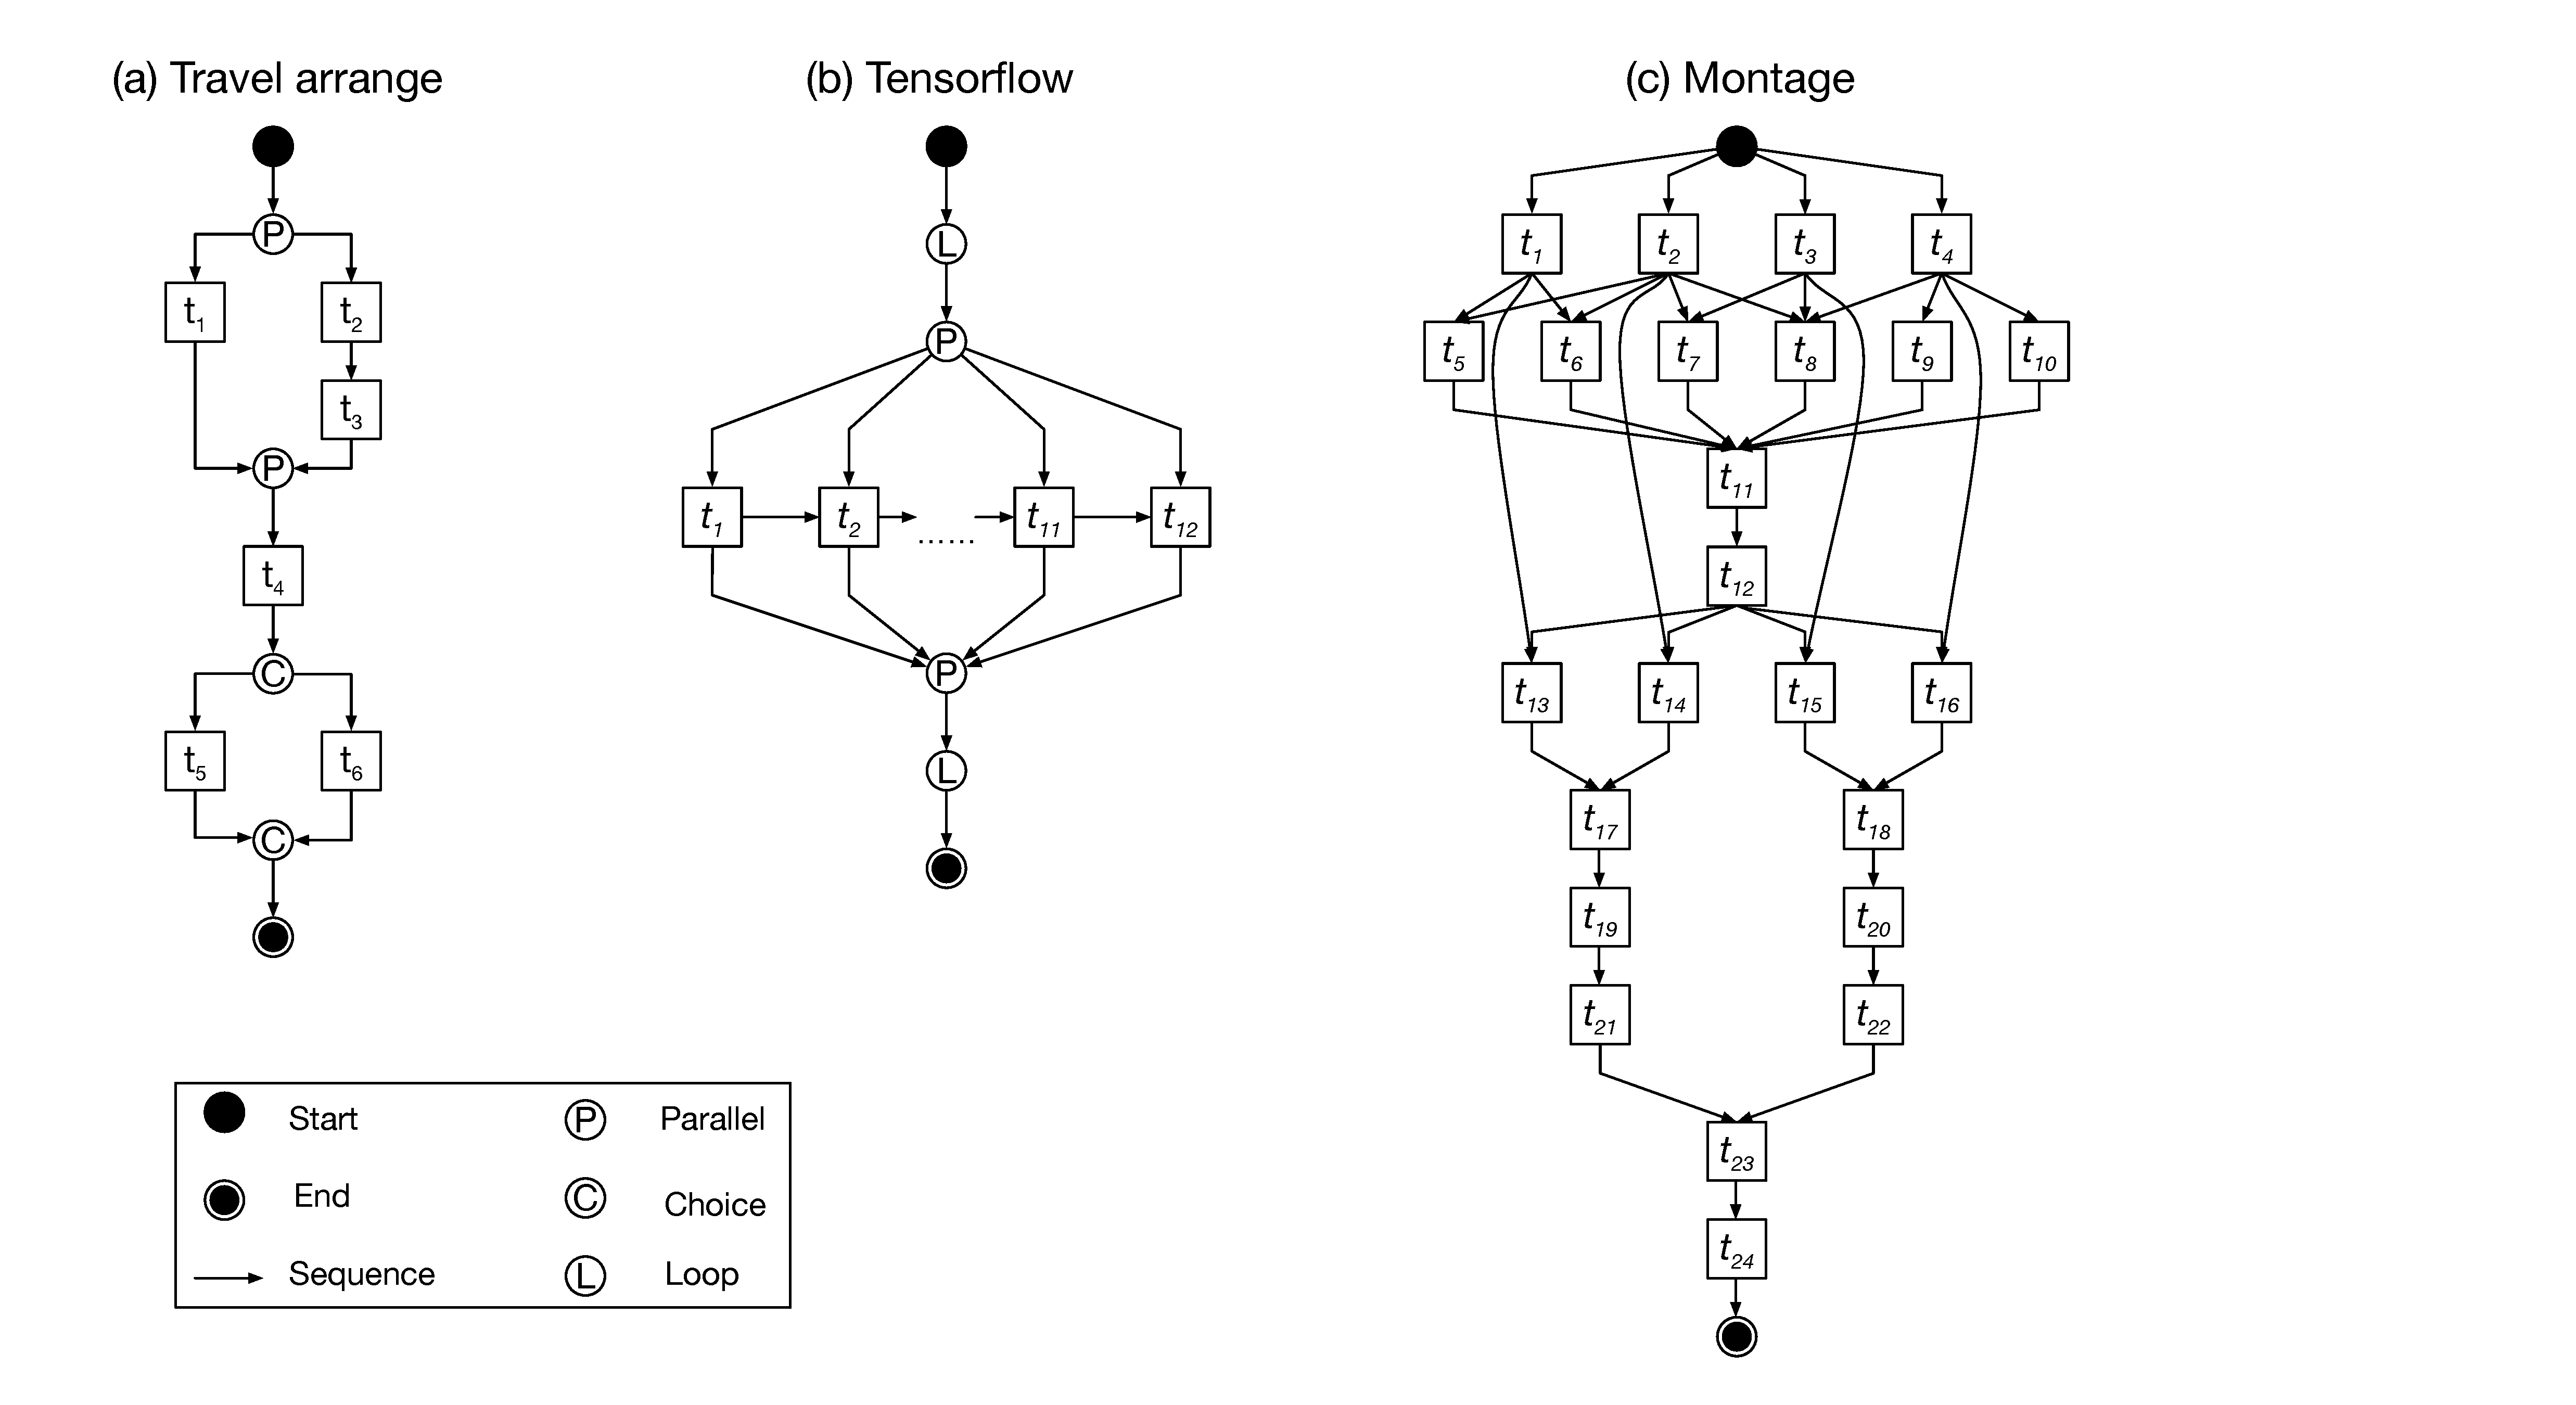
\includegraphics[width=5in]{./img/DAG.pdf}
\caption{The composition plan for case study.}
\label{fig_DAG}
\end{figure*}

%    KH_profile.NK         = 20;
%    KH_profile.MI         = 30;
%    KH_profile.CR         = 0.6;
%    KH_profile.Vf         = 0.8;
%    KH_profile.Nmax       = 0.3;
%    KH_profile.Dmax       = 0.2;
Fig. 7(a) shows the impact of population size, we observe that with the increase of population size, the average response time significantly improved before $PS=10$, and no significant improvement is observed after population size over $20$. Therefore, an excessively large population size (e.g., $PS=50$) has limited impact on the performance of KH, and it will result in computing resources waste and high time cost.
Similarly, Fig. 7(b) shows that the value of response time increased for higher number of iteration times until to a limit: $MI = 30$. 
Fig. 7(c) shows the impact of the crossover rate $Cr$. The performance of KH increases with $Cr$ firstly, then decrease, the best performance is achieved for $Cr = 0.6$.
Fig. 7(d) shows the impact of the foraging speed $V_f$. The performance of KH increases with $V_f$ firstly, then decrease, the best performance is achieved for $V_f = 0.8$.
Fig. 7(e) shows the impact of the induced speed $N_{max}$. The performance of KH increases with $N_{max}$ firstly, then decrease, the best performance is achieved for $N_{max} = 0.3$.
Fig. 7(f) shows the impact of the physical diffusion speed $D_{max}$. It shows that with the increase of $D_{max}$, the performance of KH fluctuation irregularly and slightly, we random generate $D_{max}$ from $[0.2 \sim 0.5]$ in this paper.

\subsection{Case study}
In this subsection, we present a case study of different composite mobile service in mobile environment, to compare representative non-availability algorithm proposed in \cite{Deng2017} \cite{sadiq2015service}. Fig. 7 shows three mobile service composition plans for case study. Fig. 8(a) is a well known composition plan for booking tickets \cite{wu2013transactional}, it has 6 tasks. Fig. 8(b) is a simple workflow with 12 tasks for Tensorflow \cite{abadi2016tensorflow}, Tensorflow is a heterogeneous distributed system for machine learning and it already can be deployed in mobile devices. Fig. 8(c) is a scientific workflow with 24 tasks for Montage. Montage is an astronomical image mosaic engine, it can be used for simulating some picture edit application in mobile phone. We use these three kinds of composition plans to represent different meaningful service composition with different tasks, eavh case was executed 50 times independently and the average performance was recorded.

\begin{figure}[!t]
\centering
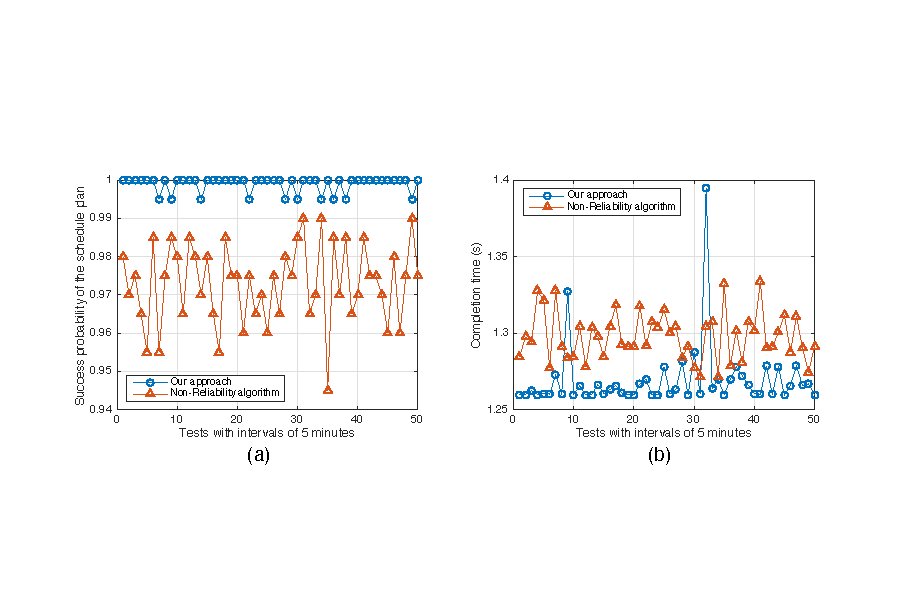
\includegraphics[width=3.3in]{./img/Task-6.pdf}
\caption{Case I}
\label{Task-6}
\end{figure}


\begin{figure}[!t]
\centering
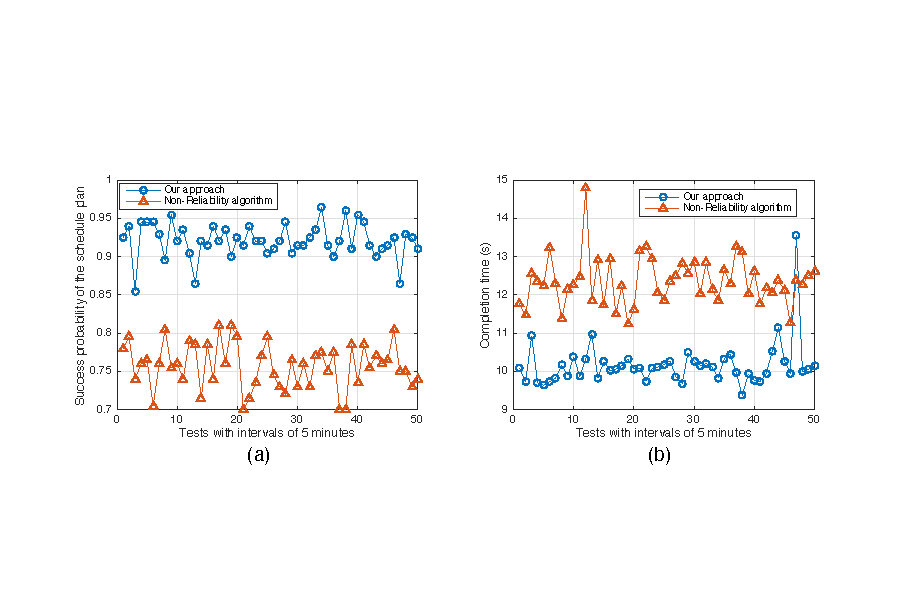
\includegraphics[width=3.3in]{./img/Task-12.pdf}
\caption{Case II}
\label{Task-12}
\end{figure}

\begin{figure}[!t]
\centering
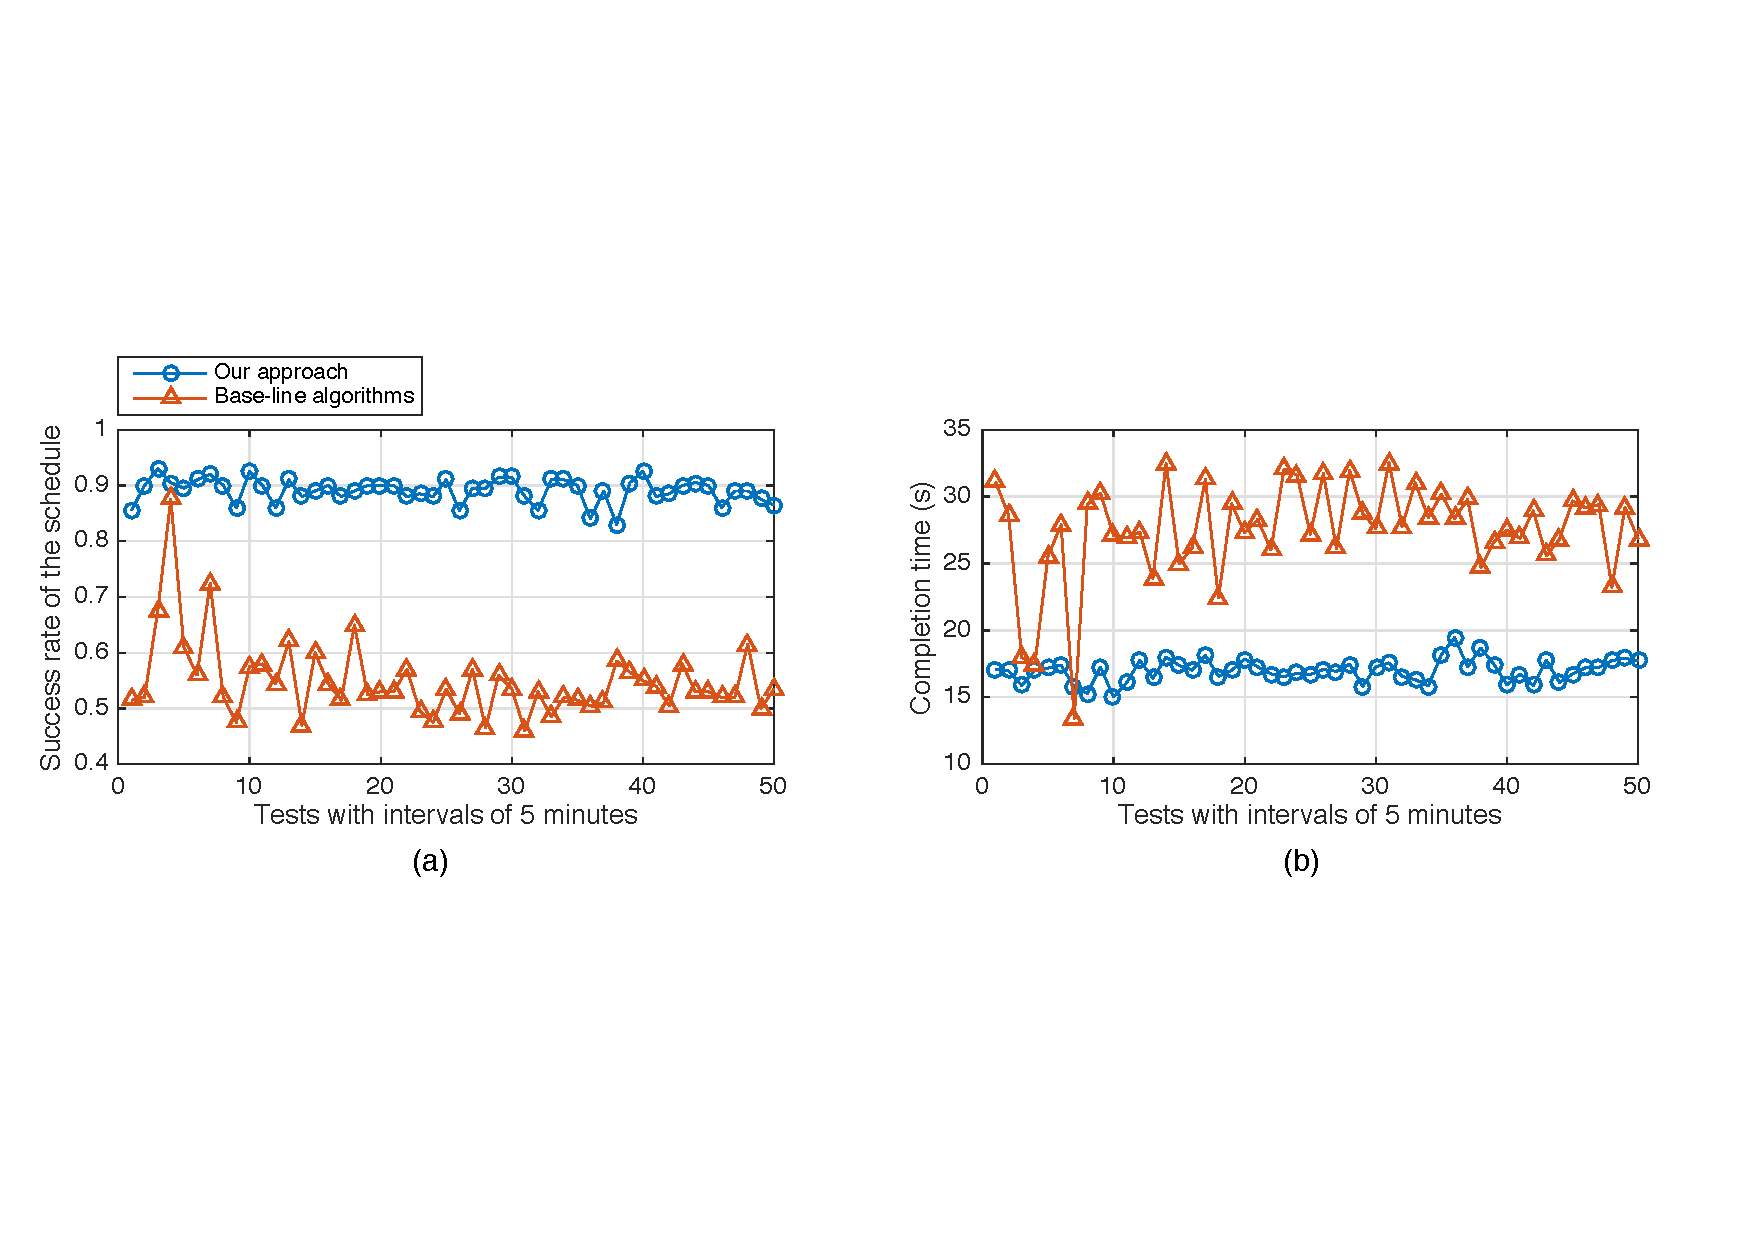
\includegraphics[width=3.3in]{./img/Task-24.pdf}
\caption{Case III}
\label{Task-24}
\end{figure}

As shown by Fig. 9(a), Fig. 10(a) and Fig. 11(a), our proposed method achieves higher success probability (average $99.9\%$ vs. $97.3\%$ for Case I, average $92.1\%$ vs. $75.7\%$ for Case II, and average $89\%$ vs. $54.9\%$ for Case III) compared with non-availability approach.
The average response time is shown in Fig. 9(b), Fig. 10(b) and Fig. 11(b), from the figure we can clearly our method has different different degrees of reducing response time in three cases, especially average $17.51\%$ response time reduced for Case II and average $36.68\%$ time reduced for Case III. Intuitively, the disadvantage of a non-availability approaches lie in that they consider the availability of mobile service is fully stable during execution. It therefore tends to choose a candidate service which has lower response time but with high probability becomes unavailability during execution because of users mobility.

\section{Conclusion}
In this paper, we propose a comprehensive framework for optimal mobile service composition on mobile environment. We present a mobile service opportunistic network model (MSON) that fully integrates human mobility behavior factors for mobile service provisioning and introduce an availability-aware mobile service composition model. Then we formulate the composition problem as an optimization problem to maximize the quality of service composition and propose a Krill-Herd-based algorithm to solve it. We also carry out a case study based on real-world opportunistic network and some well-known web service dataset and show that our proposed approach outperforms traditional ones, especially those who consider constant/invariable availability of mobile services, in terms of success rate and response time.

We consider the following topics for future work as well: 1) Some prediction methods (e.g., hidden Markov model and neural networks) can be used to predict user's future movement instead of our non-prediction method. Such sophisticated prediction methods may help to generate compositional schedules with further improved performance; 2) more QoS metrics (e.g., service price and service reputation) are supposed to be modeled and  analyzed; 3) this work considers hard constraints.
We intend to consider soft constraints to facilitate analysis and optimization of service-level-agreement (SLA) and introduce corresponding algorithms to generate compositional schedules. In such a context, service completion time is allowed to exceed a threshold value with a bounded given rate. 



% Can use something like this to put references on a page
% by themselves when using endfloat and the captionsoff option.
\ifCLASSOPTIONcaptionsoff
  \newpage
\fi




\bibliography{mybibtex}
\bibliographystyle{IEEEtran}
\end{document}


